%===============================================================================
% LaTeX sjabloon voor de bachelorproef toegepaste informatica aan HOGENT
% Meer info op https://github.com/HoGentTIN/latex-hogent-report
%===============================================================================

\documentclass[dutch,dit,thesis]{hogentreport}

% TODO:
% - If necessary, replace the option `dit`' with your own department!
%   Valid entries are dbo, dbt, dgz, dit, dlo, dog, dsa, soa
% - If you write your thesis in English (remark: only possible after getting
%   explicit approval!), remove the option "dutch," or replace with "english".

%\usepackage{lipsum} % For blind text, can be removed after adding actual content

%% Pictures to include in the text can be put in the graphics/ folder
\graphicspath{{../graphics/}}

%% For source code highlighting, requires pygments to be installed
%% Compile with the -shell-escape flag!
%% \usepackage[chapter]{minted}
%% If you compile with the make_thesis.{bat,sh} script, use the following
%% import instead:
\usepackage[chapter,outputdir=../output]{minted}
\usemintedstyle{solarized-light}

%% Formatting for minted environments.
\setminted{%
    autogobble,
    frame=lines,
    breaklines,
    linenos,
    tabsize=4
}

%% Ensure the list of listings is in the table of contents
\renewcommand\listoflistingscaption{%
    \IfLanguageName{dutch}{Lijst van codefragmenten}{List of listings}
}
\renewcommand\listingscaption{%
    \IfLanguageName{dutch}{Codefragment}{Listing}
}
\renewcommand*\listoflistings{%
    \cleardoublepage\phantomsection\addcontentsline{toc}{chapter}{\listoflistingscaption}%
    \listof{listing}{\listoflistingscaption}%
}

% Other packages not already included can be imported here

%%---------- Document metadata -------------------------------------------------
% TODO: Replace this with your own information
\author{Charan Chander}
\supervisor{Dhr. P. Maenhaut}
\cosupervisor{Dhr. L. De Jaeger}
\title[]%
    {Hoe kan een Secure Access Service Edge (SASE) architectuur worden geïmplementeerd binnen de hybride cloudomgeving van een software agency bedrijf, onderzoek en proof of concept.}
\academicyear{\advance\year by -1 \the\year--\advance\year by 1 \the\year}
\examperiod{1}
\degreesought{\IfLanguageName{dutch}{Professionele bachelor in de toegepaste informatica}{Bachelor of applied computer science}}
\partialthesis{false} %% To display 'in partial fulfilment'
%\institution{Internshipcompany BVBA.}

%% Add global exceptions to the hyphenation here
\hyphenation{back-slash}

%% The bibliography (style and settings are  found in hogentthesis.cls)
\addbibresource{bachproef.bib}            %% Bibliography file
\addbibresource{../voorstel/voorstel.bib} %% Bibliography research proposal
\defbibheading{bibempty}{}

%% Prevent empty pages for right-handed chapter starts in twoside mode
\renewcommand{\cleardoublepage}{\clearpage}

\renewcommand{\arraystretch}{1.2}

%% Content starts here.
\begin{document}

%---------- Front matter -------------------------------------------------------

\frontmatter

\hypersetup{pageanchor=false} %% Disable page numbering references
%% Render a Dutch outer title page if the main language is English
\IfLanguageName{english}{%
    %% If necessary, information can be changed here
    \degreesought{Professionele Bachelor toegepaste informatica}%
    \begin{otherlanguage}{dutch}%
       \maketitle%
    \end{otherlanguage}%
}{}

%% Generates title page content
\maketitle
\hypersetup{pageanchor=true}

%%=============================================================================
%% Voorwoord
%%=============================================================================

\chapter*{\IfLanguageName{dutch}{Woord vooraf}{Preface}}%
\label{ch:voorwoord}

%% TODO:
%% Het voorwoord is het enige deel van de bachelorproef waar je vanuit je
%% eigen standpunt (``ik-vorm'') mag schrijven. Je kan hier bv. motiveren
%% waarom jij het onderwerp wil bespreken.
%% Vergeet ook niet te bedanken wie je geholpen/gesteund/... heeft

\lipsum[1-2]
%%=============================================================================
%% Samenvatting
%%=============================================================================

% TODO: De "abstract" of samenvatting is een kernachtige (~ 1 blz. voor een
% thesis) synthese van het document.
%
% Een goede abstract biedt een kernachtig antwoord op volgende vragen:
%
% 1. Waarover gaat de bachelorproef?
% 2. Waarom heb je er over geschreven?
% 3. Hoe heb je het onderzoek uitgevoerd?
% 4. Wat waren de resultaten? Wat blijkt uit je onderzoek?
% 5. Wat betekenen je resultaten? Wat is de relevantie voor het werkveld?
%
% Daarom bestaat een abstract uit volgende componenten:
%
% - inleiding + kaderen thema
% - probleemstelling
% - (centrale) onderzoeksvraag
% - onderzoeksdoelstelling
% - methodologie
% - resultaten (beperk tot de belangrijkste, relevant voor de onderzoeksvraag)
% - conclusies, aanbevelingen, beperkingen
%
% LET OP! Een samenvatting is GEEN voorwoord!

%%---------- Nederlandse samenvatting -----------------------------------------
%
% TODO: Als je je bachelorproef in het Engels schrijft, moet je eerst een
% Nederlandse samenvatting invoegen. Haal daarvoor onderstaande code uit
% commentaar.
% Wie zijn bachelorproef in het Nederlands schrijft, kan dit negeren, de inhoud
% wordt niet in het document ingevoegd.

\IfLanguageName{english}{%
\selectlanguage{dutch}
\chapter*{Samenvatting}
\lipsum[1-4]
\selectlanguage{english}
}{}

%%---------- Samenvatting -----------------------------------------------------
% De samenvatting in de hoofdtaal van het document

\chapter*{\IfLanguageName{dutch}{Samenvatting}{Abstract}}

\lipsum[1-4]


%---------- Inhoud, lijst figuren, ... -----------------------------------------

\tableofcontents

% In a list of figures, the complete caption will be included. To prevent this,
% ALWAYS add a short description in the caption!
%
%  \caption[short description]{elaborate description}
%
% If you do, only the short description will be used in the list of figures

%\listoffigures

% If you included tables and/or source code listings, uncomment the appropriate
% lines.
%\listoftables

%\listoflistings

% Als je een lijst van afkortingen of termen wil toevoegen, dan hoort die
% hier thuis. Gebruik bijvoorbeeld de ``glossaries'' package.
% https://www.overleaf.com/learn/latex/Glossaries

%---------- Kern ---------------------------------------------------------------

\mainmatter{}

% De eerste hoofdstukken van een bachelorproef zijn meestal een inleiding op
% het onderwerp, literatuurstudie en verantwoording methodologie.
% Aarzel niet om een meer beschrijvende titel aan deze hoofdstukken te geven of
% om bijvoorbeeld de inleiding en/of stand van zaken over meerdere hoofdstukken
% te verspreiden!

%%=============================================================================
%% Inleiding
%%=============================================================================

\chapter{\IfLanguageName{dutch}{Inleiding}{Introduction}}%
\label{ch:inleiding}

% De inleiding moet de lezer net genoeg informatie verschaffen om het onderwerp te begrijpen en in te zien waarom de onderzoeksvraag de moeite waard is om te onderzoeken. In de inleiding ga je literatuurverwijzingen beperken, zodat de tekst vlot leesbaar blijft. Je kan de inleiding verder onderverdelen in secties als dit de tekst verduidelijkt. Zaken die aan bod kunnen komen in de inleiding~\autocite{Pollefliet2011}:

% \begin{itemize}
%   \item context, achtergrond
%   \item afbakenen van het onderwerp
%   \item verantwoording van het onderwerp, methodologie
%   \item probleemstelling
%   \item onderzoeksdoelstelling
%   \item onderzoeksvraag
%   \item \ldots
% \end{itemize}

In een tijdperk waarin digitale transformatie en hybride cloudomgevingen de norm zijn geworden, is een geïntegreerde aanpak van netwerk en beveiliging centraal komen te staan voor softwarebedrijven. 
Traditionele netwerkmodellen, gebaseerd op perimeterbescherming via firewalls en VPNs, volstaan niet langer in een wereld van directe cloud-toegang, telewerken en verspreide applicaties. 

\vspace{2ex}

SASE (Secure Access Service Edge) biedt een geïntegreerd framework dat netwerk- en beveiligingsfuncties combineert in één cloudgebaseerd servicemodel. Voor softwarebedrijven met gevoelige klantdata, is deze aanpak essentieel om compliance te waarborgen en vertrouwen te behouden.

\vspace{2ex}

In dit onderzoek wordt de implementatie van een SASE (Secure Access Service Edge) oplossing, met de focus op Netskope, onderzocht.
\section{\IfLanguageName{dutch}{Probleemstelling}{Problem Statement}}%
\label{sec:probleemstelling}

% Uit je probleemstelling moet duidelijk zijn dat je onderzoek een meerwaarde heeft voor een concrete doelgroep. De doelgroep moet goed gedefinieerd en afgelijnd zijn. Doelgroepen als ``bedrijven,'' ``KMO's'', systeembeheerders, enz.~zijn nog te vaag. Als je een lijstje kan maken van de personen/organisaties die een meerwaarde zullen vinden in deze bachelorproef (dit is eigenlijk je steekproefkader), dan is dat een indicatie dat de doelgroep goed gedefinieerd is. Dit kan een enkel bedrijf zijn of zelfs één persoon (je co-promotor/opdrachtgever).

Het onderzochte softwarebedrijf is gespecialiseerd in digitale producten. Het kampt met toenemende uitdagingen rond netwerktoegang en security in zijn hybride cloudinfrastructuur.

\vspace{2ex}

\textbf{Specifieke pijnpunten zijn:}

\begin{itemize}
  \item User \& Device: Authenticatie en autorisatie van gebruikers en apparaten.
	\item Application \& Workload: Applicatie-specifieke toegangscontrole en monitoring.
  \item Data: Databescherming en classificatie
  \item Connectivity: veilige verbinding tussen cloud- en at home-omgevingen.
\end{itemize}

Om deze uitdagingen aan te pakken, heeft het bedrijf gekozen voor het Netskopeplatform om een SASE-architectuur te implementeren. Deze keuze vereist echter een gedetailleerd inzicht in de technische mogelijkheden van Netskope en een op maat gemaakte implementatiestrategie die zowel netwerk- als beveiligingsaspecten integreert.

\section{\IfLanguageName{dutch}{Onderzoeksvraag}{Research question}}%
\label{sec:onderzoeksvraag}

% Wees zo concreet mogelijk bij het formuleren van je onderzoeksvraag. Een onderzoeksvraag is trouwens iets waar nog niemand op dit moment een antwoord heeft (voor zover je kan nagaan). Het opzoeken van bestaande informatie (bv. ``welke tools bestaan er voor deze toepassing?'') is dus geen onderzoeksvraag. Je kan de onderzoeksvraag verder specifiëren in deelvragen. Bv.~als je onderzoek gaat over performantiemetingen, dan 

Hoe kan een SASE-architectuur worden geïmplementeerd binnen de hybride cloudomgeving van een softwarebedrijf gebruikmakend van het Netskope platform?

\vspace{2ex}

Deze vraag wordt opgesplitst in probleem- en oplossingsdomein:

\textbf{Probleemdomein}
\begin{itemize}
  \item Welke netwerk- en security-uitdagingen in de huidige infrastructuur kunnen worden aangepakt via Netskope's SASE-functionaliteiten?
  \item Welke tekortkomingen in de huidige perimeterbeveiliging vereisen een Zero Trust-aanpak?
\end{itemize}

\vspace{2ex}

\textbf{Oplossingsdomein}
\begin{itemize}
  \item Welke Netskope-componenten zijn nodig voor een succesvolle implementatie?
  \item Hoe kan Netskope geoptimaliseerd worden voor een hybride omgeving, inclusief integratie met bestaande systemen?
\end{itemize}

\vspace{2ex}

\textbf{Deelvragen}
\begin{itemize}
  \item Wat is de huidige situatie van het bedrijf op vlak van security en welke risico’s zijn er?
  \item Welke Netskope-functionaliteiten zijn relevant voor de implementatie van Zero Trust?
  \item Hoe kan Netskope geïntegreerd worden met bestaande systemen en processen?
  \item Hoe kan de implementatie van Netskope gevalideerd worden?
\end{itemize}

\section{\IfLanguageName{dutch}{Onderzoeksdoelstelling}{Research objective}}%
\label{sec:onderzoeksdoelstelling}

% Wat is het beoogde resultaat van je bachelorproef? Wat zijn de criteria voor succes? Beschrijf die zo concreet mogelijk. Gaat het bv.\ om een proof-of-concept, een prototype, een verslag met aanbevelingen, een vergelijkende studie, enz.

Het doel van deze proef is het ontwikkelen van een proof of concept dat de haalbaarheid en voordelen van de SASE-architectuur aantoont. Het resultaat gaat verder dan een geschreven scriptie en omvat dus ook een implementatie die de werking van het systeem aantoont.

\vspace{2ex}

Deze PoC zal worden geëvalueerd door de interne IT afdeling in de laatste 2 weken van dit onderzoek.

\section{\IfLanguageName{dutch}{Opzet van deze bachelorproef}{Structure of this bachelor thesis}}%
\label{sec:opzet-bachelorproef}

% Het is gebruikelijk aan het einde van de inleiding een overzicht te
% geven van de opbouw van de rest van de tekst. Deze sectie bevat al een aanzet
% die je kan aanvullen/aanpassen in functie van je eigen tekst.

De rest van deze bachelorproef is als volgt opgebouwd:

\vspace{2ex}

In Hoofdstuk~\ref{ch:literatuurstudie} wordt een overzicht gegeven van de stand van zaken binnen het onderzoeksdomein, op basis van een literatuurstudie.

\vspace{2ex}

In Hoofdstuk~\ref{ch:methodologie} wordt de methodologie toegelicht en worden de gebruikte onderzoekstechnieken besproken om een antwoord te kunnen formuleren op de onderzoeksvragen.

\vspace{2ex}

In Hoofdstuk~\ref{ch:requirements analyse} worden de functionele en niet-functionele vereisten voor de SASE-architectuur in de hybride cloudomgeving van het softwarebedrijf geanalyseerd. Dit hoofdstuk legt de basis voor de implementatie door de specifieke behoeften en beperkingen van het bedrijf te identificeren.

\vspace{2ex}

In Hoofdstuk~\ref{ch:proof of concept preparation} wordt de voorbereiding van de proof of concept besproken, inclusief de technische vereisten en de opzet van de implementatie.

\vspace{2ex}

In Hoofdstuk~\ref{ch:proof of concept implementation} wordt de implementatie van de proof of concept besproken, met aandacht voor de uitvoering en de behaalde resultaten.

\vspace{2ex}

In Hoofdstuk~\ref{ch:resultaten} worden de resultaten van de proof of concept gepresenteerd en geanalyseerd, met een focus op de effectiviteit van de SASE-architectuur in de hybride cloudomgeving.

\vspace{2ex}

In Hoofdstuk~\ref{ch:conclusie}, tenslotte, wordt de conclusie gegeven en een antwoord geformuleerd op de onderzoeksvragen. Daarbij wordt ook een aanzet gegeven voor toekomstig onderzoek binnen dit domein.
\chapter{\IfLanguageName{dutch}{Stand van zaken}{State of the art}}%
\label{ch:stand-van-zaken}

% Tip: Begin elk hoofdstuk met een paragraaf inleiding die beschrijft hoe
% dit hoofdstuk past binnen het geheel van de bachelorproef. Geef in het
% bijzonder aan wat de link is met het vorige en volgende hoofdstuk.

% Pas na deze inleidende paragraaf komt de eerste sectiehoofding.

% Dit hoofdstuk bevat je literatuurstudie. De inhoud gaat verder op de inleiding, maar zal het onderwerp van de bachelorproef *diepgaand* uitspitten. De bedoeling is dat de lezer na lezing van dit hoofdstuk helemaal op de hoogte is van de huidige stand van zaken (state-of-the-art) in het onderzoeksdomein. Iemand die niet vertrouwd is met het onderwerp, weet nu voldoende om de rest van het verhaal te kunnen volgen, zonder dat die er nog andere informatie moet over opzoeken \autocite{Pollefliet2011}.

% Je verwijst bij elke bewering die je doet, vakterm die je introduceert, enz.\ naar je bronnen. In \LaTeX{} kan dat met het commando \texttt{$\backslash${textcite\{\}}} of \texttt{$\backslash${autocite\{\}}}. Als argument van het commando geef je de ``sleutel'' van een ``record'' in een bibliografische databank in het Bib\LaTeX{}-formaat (een tekstbestand). Als je expliciet naar de auteur verwijst in de zin (narratieve referentie), gebruik je \texttt{$\backslash${}textcite\{\}}. Soms is de auteursnaam niet expliciet een onderdeel van de zin, dan gebruik je \texttt{$\backslash${}autocite\{\}} (referentie tussen haakjes). Dit gebruik je bv.~bij een citaat, of om in het bijschrift van een overgenomen afbeelding, broncode, tabel, enz. te verwijzen naar de bron. In de volgende paragraaf een voorbeeld van elk.

% \textcite{Knuth1998} schreef een van de standaardwerken over sorteer- en zoekalgoritmen. Experten zijn het erover eens dat cloud computing een interessante opportuniteit vormen, zowel voor gebruikers als voor dienstverleners op vlak van informatietechnologie~\autocite{Creeger2009}.

% Let er ook op: het \texttt{cite}-commando voor de punt, dus binnen de zin. Je verwijst meteen naar een bron in de eerste zin die erop gebaseerd is, dus niet pas op het einde van een paragraaf.

% \begin{figure}
%   \centering
%   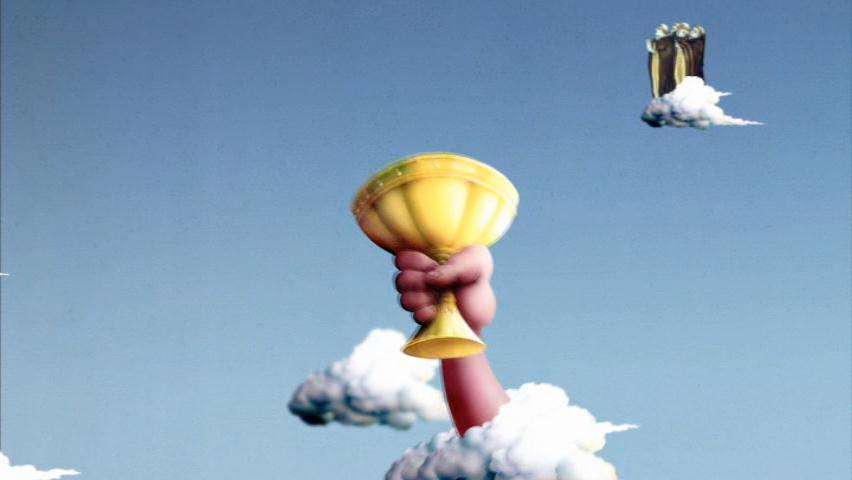
\includegraphics[width=0.8\textwidth]{grail.jpg}
%   \caption[Voorbeeld figuur.]{\label{fig:grail}Voorbeeld van invoegen van een figuur. Zorg altijd voor een uitgebreid bijschrift dat de figuur volledig beschrijft zonder in de tekst te moeten gaan zoeken. Vergeet ook je bronvermelding niet!}
% \end{figure}

% \begin{listing}
%   \begin{minted}{python}
%     import pandas as pd
%     import seaborn as sns

%     penguins = sns.load_dataset('penguins')
%     sns.relplot(data=penguins, x="flipper_length_mm", y="bill_length_mm", hue="species")
%   \end{minted}
%   \caption[Voorbeeld codefragment]{Voorbeeld van het invoegen van een codefragment.}
% \end{listing}

% \lipsum[7-20]

% \begin{table}
%   \centering
%   \begin{tabular}{lcr}
%     \toprule
%     \textbf{Kolom 1} & \textbf{Kolom 2} & \textbf{Kolom 3} \\
%     $\alpha$         & $\beta$          & $\gamma$         \\
%     \midrule
%     A                & 10.230           & a                \\
%     B                & 45.678           & b                \\
%     C                & 99.987           & c                \\
%     \bottomrule
%   \end{tabular}
%   \caption[Voorbeeld tabel]{\label{tab:example}Voorbeeld van een tabel.}
% \end{table}

Als modern IT bedrijf is het belangrijk om de veiligheid van de data te garanderen. Dit is een van de redenen waarom het bedrijf heeft gekozen voor een Zero Trust Netwerkarchitectuur. 
Deze studie onderzoekt de implementatie van een Zero Trust Netwerkarchitectuur en een least privileged access model binnen de hybride cloudomgeving van een softwarebedrijf gebruikmakend van het netskope platform.
Als eerste stap in dit onderzoek is het belangrijk om de huidige situatie van het bedrijf te analyseren. Dit omvat een overzicht van de huidige security-risico’s en tekortkomingen in de huidige perimeterbeveiliging.
Dit wordt gedaan door een analyse van de huidige infrastructuur en de security-risico’s die hiermee gepaard gaan. Alsook door interviews met de IT-afdeling en de security-afdeling van het bedrijf.

Zero Trust is een steeds belangrijker wordend model voor netwerkbeveiliging, vooral in omgevingen waar gevoelige data verwerkt wordt. 
Het model is gebaseerd op de stelling dat geen enkel apparaat, gebruiker of systeem automatisch te vertrouwen is, zelfs niet als deze zich binnen het netwerk bevinden. 
De nadruk ligt op het continu verifiëren van gebruikersidentiteit, het beperken van toegang tot strikt noodzakelijke bronnen (least privileged access), en het monitoren van netwerkactiviteiten om verdachte handelingen snel te identificeren en aan te pakken.

Netskope, het platform dat het bedrijf heeft gekozen voor hun Zero Trust implementatie, definieert Zero Trust als een beveiligingsmodel waarbij niemand blind vertrouwd wordt binnen het netwerk of toegang krijgt tot resources, applicaties of data totdat ze gevalideerd zijn als legitieme gebruiker met een legitieme behoefte~\autocite{Netskope2020}. Hun Security Service Edge (SSE) architectuur implementeert deze principes via een data-centrische aanpak gebaseerd op zes kernpijlers:

\begin{itemize}
  \item User \& Device: Authenticatie en autorisatie van gebruikers en apparaten
  \item Network \& Environment: Segmentatie en toegangscontrole op netwerkniveau
  \item Application \& Workload: Applicatie-specifieke toegangscontrole en monitoring
  \item Data: Databescherming en classificatie
  \item Visibility \& Analytics: Continue monitoring en gedragsanalyse
  \item Automation \& Orchestration: Geautomatiseerde response en integratie
\end{itemize}

Volgens Microsoft is de kern van het Zero Trust-model gebaseerd op drie belangrijke principes: altijd verifiëren, nooit vertrouwen; minimaal toegang verlenen; en schade beperken bij inbreuk. Dit houdt in dat de toegang tot systemen of data niet alleen wordt beperkt op basis van de locatie van de gebruiker of het apparaat, maar altijd afhangt van de identiteit, rol en andere specifieke toegangsbeperkingen~\autocite{Microsoft2024}. Netskope implementeert deze principes via een gelaagde aanpak met Policy Enforcement Points (PEPs) op drie niveaus:

\begin{itemize}
  \item Network/Resource PEP: Controleert netwerktoegang en basiscommunicatie
  \item Application PEP: Beheert toegang tot specifieke applicaties en workloads
  \item Data PEP: Zorgt voor databescherming en compliance
\end{itemize}

Kaspersky benadrukt het belang van de technologieën die Zero Trust mogelijk maken, zoals multi-factor authenticatie (MFA), versleuteling van communicatie en geavanceerde netwerkmonitoringtools~\autocite{Kaspersky2024}. Netskope's platform integreert deze technologieën in een uitgebreid security framework dat onder andere bestaat uit:

\begin{itemize}
  \item Device en user authenticatie via een client certificaat infrastructuur
  \item TLS-beveiligde tunneling voor alle communicatie
  \item Data Loss Prevention (DLP) met meer dan 3000 data identifiers en 1400 bestandstypes
  \item Machine learning-gebaseerde User and Entity Behavior Analytics (UEBA)
  \item Real-time threat protection met meer dan 40 threat intelligence feeds
\end{itemize}

De implementatie van Zero Trust vereist zorgvuldige planning, vooral in complexe netwerkomgevingen.

Uit onderzoek van MIT Lincoln Laboratory blijkt dat Zero Trust-architecturen bijzonder effectief zijn tegen insiderdreigingen, zoals misbruik van gecompromitteerde credentials of onbevoegde toegang door eigen medewerkers. 
Dit risico is relevant voor het onderzochte bedrijf, waar ontwikkelaars en externe partners toegang hebben tot gevoelige klantdata. 
MIT benadrukt dat een succesvolle Zero Trust-implementatie niet alleen technologische verandering vereist (zoals granular access control), maar ook organisatorische aanpassingen, zoals het trainen van medewerkers en het opstellen van duidelijk beleid voor toegangsverificatie. 
Dit sluit aan bij Netskope’s focus op User \& Device workflows en gedragsanalyse, waarbij continue verificatie van gebruikers en apparaten centraal staat. 
Tegelijkertijd waarschuwt MIT voor de complexiteit van hybride implementaties, waarbij on-premises systemen en clouddiensten geïntegreerd moeten worden—een uitdaging die het bedrijf direct ondervindt en waar Netskope’s SSE-platform een antwoord op biedt.~\autocite{MIT2022}

Netskope biedt hiervoor een gestructureerde aanpak met specifieke operationele workflows:

\begin{itemize}
  \item User/Device workflow voor initiële authenticatie en continue validatie
  \item Network/Resource workflow voor toegangscontrole en segmentatie
  \item Data Protection workflow voor databescherming en compliance
\end{itemize}

Deze workflows worden ondersteund door een automation engine die continue monitoring uitvoert op zeven dimensies van gebruikersactiviteit: tijd, dag, locatie, apparaat, service, activiteit en object. Dit zorgt voor een dynamische beveiligingsposture die zich aanpast aan veranderende omstandigheden en dreigingen~\autocite{Netskope2020}.

Het onderzoek van Mutemwa et al. levert een belangrijke bijdrage aan ons begrip van de veranderende aard van cybersecurity in een post-pandemische wereld. Hun studie bevestigt dat traditionele perimeterbescherming fundamenteel is uitgedaagd door de verschuiving naar gedistribueerde werkomgevingen.
De auteurs concluderen dat organisaties moeten evolueren van een perimeter-gebaseerd beveiligingsmodel naar een meer holistische benadering die rekening houdt met de realiteit van een uitgebreide, poreuze bedrijfsgrens. Dit vereist een heroverweging van beveiligingsarchitecturen, met grotere nadruk op identiteitsbeheer, endpoint-beveiliging en gebruikerseducatie.
Deze studie onderstreept de noodzaak voor organisaties om hun cybersecurity-strategieën aan te passen aan een wereld waarin de traditionele grenzen tussen “binnen” en “buiten” het bedrijfsnetwerk steeds vager worden, een conclusie die aansluit bij de bredere verschuiving in de richting van zero-trust beveiligingsmodellen in de cybersecurity-gemeenschap~\autocite{ACM2021}.
%%=============================================================================
%% Methodologie
%%=============================================================================

\chapter{\IfLanguageName{dutch}{Methodologie}{Methodology}}%
\label{ch:methodologie}

%% TODO: In dit hoofstuk geef je een korte toelichting over hoe je te werk bent
%% gegaan. Verdeel je onderzoek in grote fasen, en licht in elke fase toe wat
%% de doelstelling was, welke deliverables daar uit gekomen zijn, en welke
%% onderzoeksmethoden je daarbij toegepast hebt. Verantwoord waarom je
%% op deze manier te werk gegaan bent.
%% 
%% Voorbeelden van zulke fasen zijn: literatuurstudie, opstellen van een
%% requirements-analyse, opstellen long-list (bij vergelijkende studie),
%% selectie van geschikte tools (bij vergelijkende studie, "short-list"),
%% opzetten testopstelling/PoC, uitvoeren testen en verzamelen
%% van resultaten, analyse van resultaten, ...
%%
%% !!!!! LET OP !!!!!
%%
%% Het is uitdrukkelijk NIET de bedoeling dat je het grootste deel van de corpus
%% van je bachelorproef in dit hoofstuk verwerkt! Dit hoofdstuk is eerder een
%% kort overzicht van je plan van aanpak.
%%
%% Maak voor elke fase (behalve het literatuuronderzoek) een NIEUW HOOFDSTUK aan
%% en geef het een gepaste titel.

Dit onderzoek volgt een systematische aanpak die bestaat uit drie hoofdfasen: literatuuronderzoek, technische analyse en proof of concept ontwikkeling. De totale onderzoeksduur bedraagt 14 weken.

\section{Fase 1: Literatuuronderzoek (4 weken)}
Fase 1 van het project betreft een literatuuronderzoek van drie weken waarin de technische documentatie van de Netskope architectuur wordt bestudeerd. 

\vspace{2ex}

Ook externe bronnen worden bestudeerd om een beter beeld te krijgen van de SASE architectuur en de verschillende implementaties.

\section{Fase 2: Requirements analyse (1 week)}
Interviews met Team IT om de huidige situatie te analyseren, dit zal een beter inzicht geven in de huidige security risico's en de vereisten voor een Zero Trust implementatie. 
Via deze gesprekken willen we eerst begrijpen hoe het huidige netwerk is opgebouwd, inclusief hoe de verbindingen tussen kantooromgeving en cloudplatformen verlopen. We bekijken welke beveiligingsmaatregelen al aanwezig zijn en hoe goed deze werken. Ook brengen we in kaart welke beveiligingsrisico’s er zijn, vooral op het gebied van toegangsbeheer, gebruikersverificatie en gegevensbescherming.

\vspace{2ex}

Naast de interviews bekijken we ook bestaande documentatie zoals netwerktekeningen, beveiligingsbeleid en rapporten van vroegere incidenten. Door deze combinatie krijgen we een completer beeld. 

\vspace{2ex}

We letten vooral op risico’s die ontstaan door de traditionele “perimeter-gebaseerde” beveiliging, en hoe een Zero Trust aanpak binnen SASE hier verbetering in kan brengen. 

\vspace{2ex}

Deliverable: een oplijsting van de requirements en een overzicht van de huidige situatie.

\section{Fase 3: Proof of concept ontwikkeling (7 weken)}
De volgende zeven weken zijn voorzien voor de daadwerkelijke ontwikkeling van het
proof of concept. Hierbij wordt gebruik gemaakt van geschikte tools en technologieën die zijn gevonden tijdens de literatuurstudie en ontwerpfase.

\vspace{2ex}

De PoC zal aan de onderzochte requirements voldoen en zal het onderzochte probleem oplossen. 

\vspace{2ex}

De deliverable is een functioneel proof of concept van het netskope systeem.

\section{Fase 4: Validatie en evaluatie (2 weken)}
De ontwikkelde proof of concept wordt geëvalueerd en gevalideerd. Deze fase omvat testen van de functionaliteit, prestaties en
feedback van gebruikers. Eventuele aanpassingen worden doorgevoerd. 

\vspace{2ex}

De einddeliverable omvat een afgewerkt proof of concept.

\vspace{4ex}

Deze methodologie is specifiek afgestemd op de implementatie van een SASE architectuur via het Netskope platform, waarbij elke fase concrete technische deliverables oplevert. De focus ligt op het correct configureren en valideren van Netskope's security features, met voldoende tijd voor iteratie en optimalisatie van de implementatie.



% Voeg hier je eigen hoofdstukken toe die de ``corpus'' van je bachelorproef
% vormen. De structuur en titels hangen af van je eigen onderzoek. Je kan bv.
% elke fase in je onderzoek in een apart hoofdstuk bespreken.

%\input{...}
%\input{...}
%...

%%=============================================================================
%% Requirements analyse
%%=============================================================================

\chapter{\IfLanguageName{dutch}{Requirements Analyse}{Requirements Analisis}}%
\label{ch:requirements analyse}

In de eerste fase van het onderzoek staat een requirements analyse centraal, waar-
bij meerdere meetings werden gehouden met de stakeholders/leden
binnen het IT-team en vertegenwoordigers van Netskope.

\section{Must have requirements}
Uit de meetings zijn er een aantal requirements gekomen die belangrijk zijn voor een succesvolle implementatie van de SASE architectuur.

\vspace{2ex}

\textbf{Primaire must have requirements}
\begin{itemize}
  \item \textbf{Netskope client}: De Netskope client moet company wide geïmplementeerd zijn. 
  \item \textbf{DLP}: (Data Loss Prevention) Het risico dat vertrekkende werknemers gevoelige informatie meenemen moet worden voorkomen.
  \item \textbf{Privacy}: De algemene privacy van de werknemers behouden, duidelijk maken dat deze implementatie wordt gedaan met hun privacy in gedachte.
  \item \textbf{Secure access}: De toegang tot company resources beveiligen voor remote werknemers. Uiteindelijk één groot bedrijfsnetwerk waar enkel en alleen werknemers van het bedrijf zich in kunnen begeven, ongeacht hun locatie.
\end{itemize}

\vspace{2ex}

\textbf{Secundaire must have requirements}
\begin{itemize}
  \item \textbf{Bedrijfsgerichte policies}: Specifiek op maat gemaakte policies voor het bedrijf, die dan ook company wide geïmplementeerd moeten worden. Dit gaat van het blokkeren van bepaalde websites tot het beperken van het aantal gebruikte apps.
  \item \textbf{Alerting}: Het interne IT team moet op de hoogte blijven van alle beveiligingsgebeurtenissen. Denk bijvoorbeeld aan een DLP alert die wordt gegenereerd door een werknemer die gevoelige informatie downloadt voor hij vertrekt.
  \item \textbf{Gepaste documentatie}: Voor de werknemers moet het duidelijk zijn dat deze implementatie gedaan is om hun te beschermen tegen cyberdreigingen, en om het bedrijf te beschermen tegen data lekken. Ook moet het duidelijk zijn voor de werknemers welke stappen ze moeten nemen als er iets mis gaat, denk dan aan een false positive.
\end{itemize}

\section{Could have requirements}
\begin{itemize}
  \item \textbf{Duidelijk proces}: Een helder en duidelijk proces voor het interne IT team om incidenten en meldingen te verwerken. 
  \item \textbf{Automatische use case flagging}: Automatische flagging als bepaalde gebruikers patronen beginnen te vertonen die betrekking kunnen hebben tot een slechte use case. Denk dan bijvoorbeeld aan iemand die alle interne data downloadt voor hij vertrekt.
\end{itemize}

\section{Huidige situatie}
Het bedrijf kampt momenteel met meerdere problemen, werknemers die van thuis uit werken kunnen niet aan de interne apps zonder VPN, de interne IT afdeling heeft geen visibiliteit op potentiële datalekken, en er is geen centraal overzicht van alle incidenten.


%%=============================================================================
%% Proof of concept ontwikkeling
%%=============================================================================

\chapter{\IfLanguageName{dutch}{Proof of Concept voorbereiding}{Proof of Concept Preparation}}%
\label{ch:proof of concept preparation}

In dit hoofdstuk wordt de proof of concept voorbereid, deze zal aan de requirements voldoen die in hoofdstuk \ref{ch:requirements analyse} zijn opgesteld. Deze voorbereiding zal tot stand komen door middel van de vergaarde kennis uit het literatuuronderzoek en de interviews met de stakeholders.

\section{Nodige Netskope componenten}

In deze sectie worden de nodige Netskope componenten voor de proof of concept ontwikkeling besproken.

\subsection{Netskope Client}
De Netskope Client is een lichtgewicht applicatie die netwerkverkeer van eindgebruikersapparaten naar de Netskope Cloud stuurt, waar beveiligingsoplossingen zoals de Secure Web Gateway (SWG), Zero Trust Network Access (ZTNA) en Cloud Access Security Broker (CASB) worden toegepast. De Client werkt via een forward proxy-mechanisme waarbij een SSL-tunnel wordt opgezet tussen het apparaat van de gebruiker en de Netskope proxy in de cloud. De te sturen applicaties en domeinen worden centraal geconfigureerd in de Netskope admin console en deze configuratie wordt automatisch verspreid en bijgewerkt op alle geïnstalleerde Clients. Tijdens de installatie worden alle benodigde CA-certificaten toegevoegd aan het systeem om correcte SSL-terminatie te waarborgen.
De Netskope Client ondersteunt diverse besturingssystemen, waaronder Windows, macOS, Linux, Android, iOS en Chrome OS. De uitrol kan plaatsvinden via verschillende methoden, zoals e-mailuitnodigingen, integratie met Identity Providers, of device management-platformen zoals Microsoft Intune, JAMF en VMware Workspace ONE. Na installatie zorgt de Client voor zichtbaarheid en beleidsafdwinging op zowel beheerde als onbeheerde applicaties, ongeacht de locatie van de gebruiker.~\autocite{Netskope2025-8}

\subsection{Netskope Next Gen Secure Web Gateway (SWG)}
Een Secure Web Gateway (SWG) is ontwikkeld om webverkeer te beveiligen, ongewenste inhoud te filteren en gevoelige gegevens te beschermen. Netskope's Next-Gen SWG gaat verder door niet alleen webverkeer te beheren, maar ook uitgebreide zichtbaarheid en controle te bieden over het gebruik van cloud-applicaties en datastromen.
Deze oplossing richt zich specifiek op het detecteren van bedreigingen en het afdwingen van beveiligingsbeleid voor zowel web- als cloudomgevingen, met behoud van netwerkprestaties en betrouwbaarheid.~\autocite{Netskope2025-3}

\subsection{Netskope Cloud Access Security Broker (CASB)}
Een Cloud Access Security Broker (CASB) is een beveiligingsoplossing die zichtbaarheid, controle en bescherming biedt voor cloudapplicaties en -diensten. Netskope's CASB heeft diepgaande integraties met populaire cloudplatformen zoals Microsoft 365, Google Workspace, Salesforce, en Slack.

Het biedt real-time inzicht in gebruikersactiviteiten en datastromen binnen zowel persoonlijke als zakelijke accounts van cloudapplicaties zoals Dropbox, Box en GitHub.~\autocite{Netskope2025-4}

\subsection{Netskope Zero Trust Network Access (ZTNA)}
Zero Trust Network Access (ZTNA) is een beveiligingsframework dat gebruikers veilig verbindt met bedrijfsapplicaties op basis van het zero trust-model. Dit model gaat uit van het principe dat geen enkele gebruiker of apparaat automatisch wordt vertrouwd, ongeacht locatie of netwerk. Netskope’s ZTNA implementeert dit door toegang te beperken tot specifieke applicaties in plaats van volledige netwerktoegang te verlenen. In plaats van netwerktoegang biedt ZTNA alleen toegang tot specifieke, geautoriseerde applicaties. Dit voorkomt ongeautoriseerde laterale bewegingen binnen het netwerk. Een cloudgebaseerde ZTNA-broker verifieert de identiteit en beveiligingsstatus van gebruikers en apparaten voordat toegang wordt verleend. Bedrijfsapplicaties blijven onzichtbaar voor onbevoegde gebruikers, waardoor de digitale aanvalsoppervlakte aanzienlijk wordt verkleind. ZTNA elimineert traditionele kwetsbaarheden zoals inkomende netwerkverbindingen en biedt een veiliger alternatief door applicatiespecifieke toegang te combineren met een verbeterde gebruikerservaring en een gereduceerd risico op aanvallen.~\autocite{Netskope2025-5}

\subsection{Netskope Publisher}
Een Netskope publisher is een beveiligingsoplossing die remote werknemers toegang verleent tot private cloudapplicaties en -diensten zoals Microsoft 365, Google Workspace en Salesforce. Het werkt als een gateway tussen gebruikers en privé-applicaties, waardoor veilige en directe toegang mogelijk wordt zonder de noodzaak van traditionele VPN-oplossingen~\autocite{Netskope2025-6}~\autocite{Netskope2025-7}.

\section{Netskope architectuur}
Dit is een algemeen overzicht van de architectuur en layout van de proof of concept. 
\begin{figure}
    \centering
    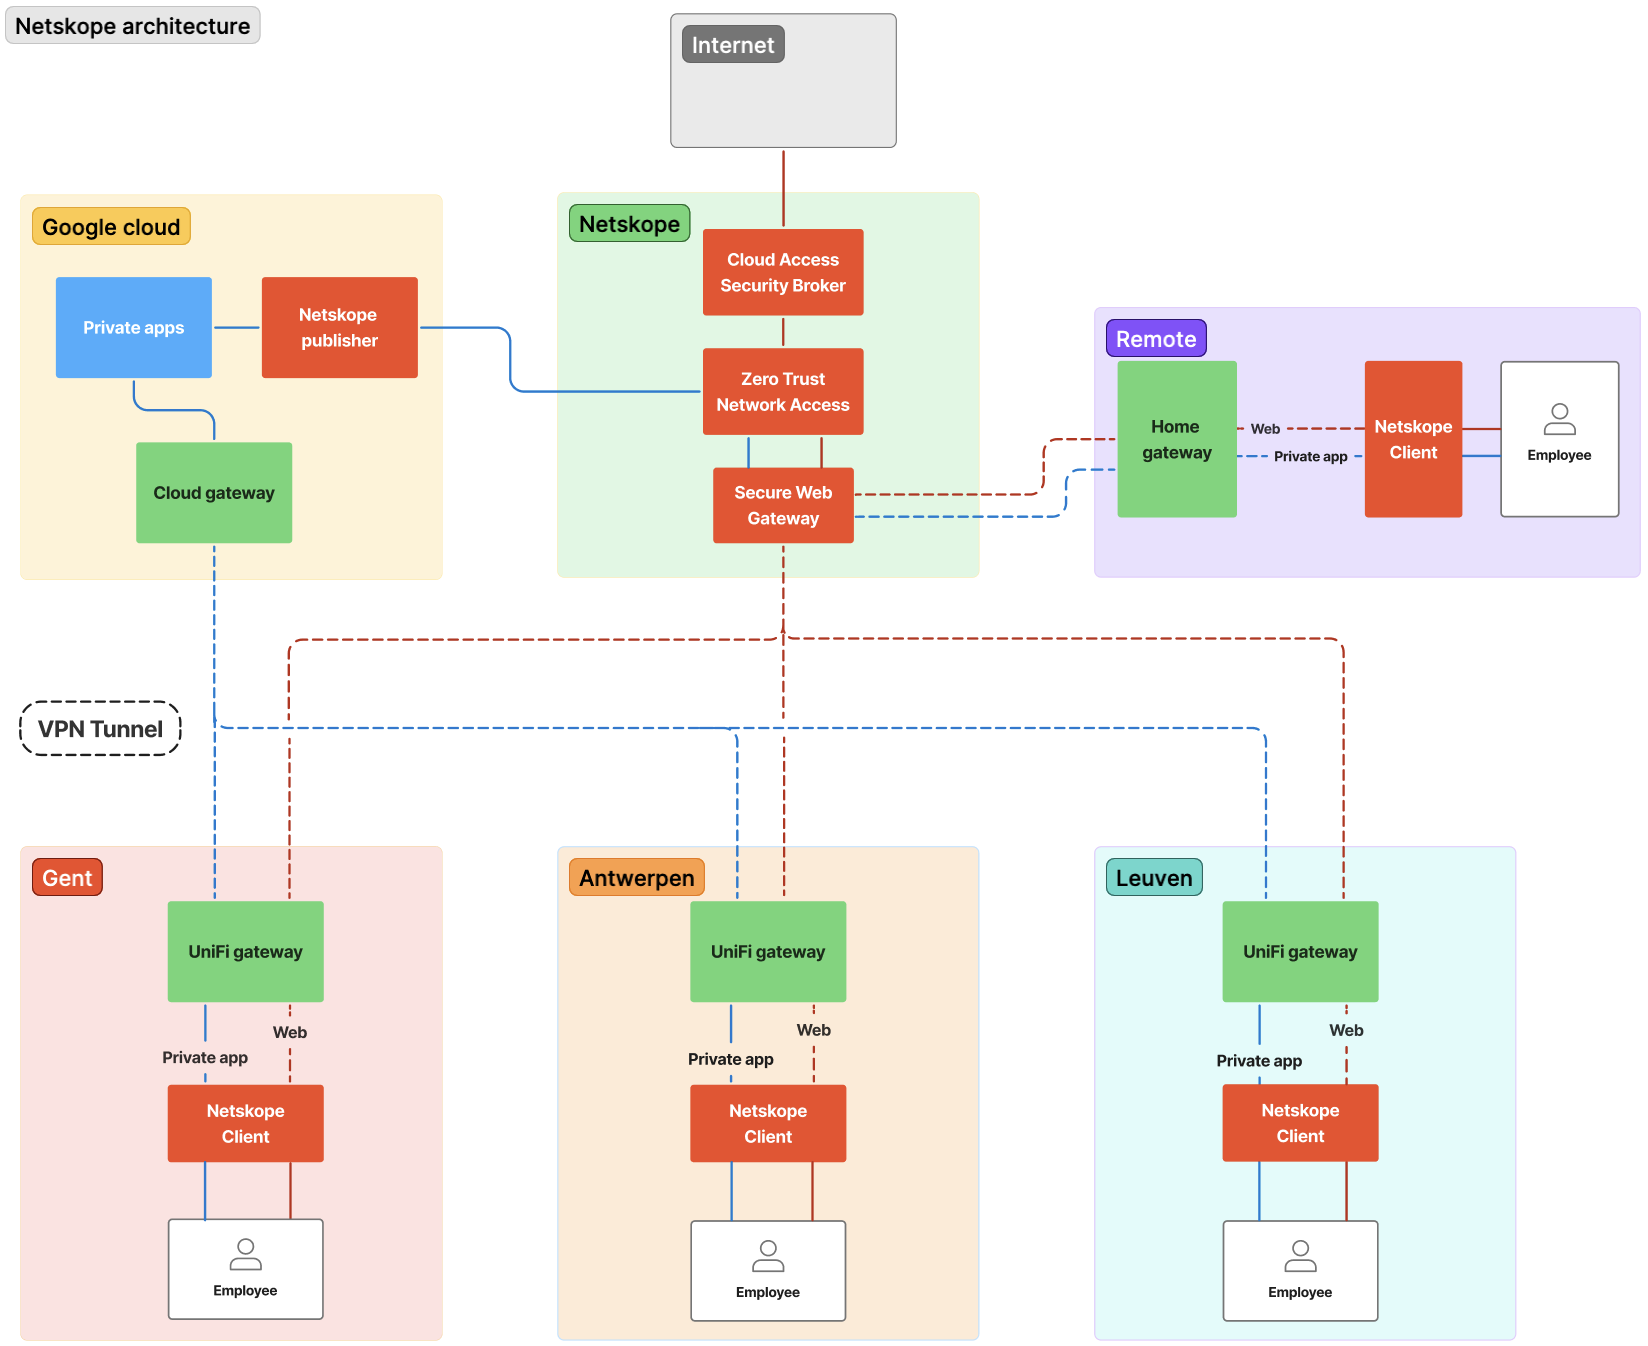
\includegraphics[width=1\textwidth]{Netskope-architecture.png}
    \caption[]{Architectuur van de proof of concept}
    \label{fig:poc-architecture}
\end{figure}
  
\subsection{Google Cloud}
Het bedrijf gebruikt Google Cloud als cloudprovider. Binnen Google Cloud worden de private apps van het bedrijf gehost. De Netskope Publisher wordt binnen de Google Cloud omgeving geplaatst om deze private apps remote beschikbaar te stellen.

\subsection{Netskope Cloud}
De Netskope Cloud is de cloudomgeving van Netskope waarin de nodige Netskope componenten zich bevinden. De Netskope client verbind met de cloud via een SSL tunnel.

\subsection{Gent, Antwerpen en Leuven}
Op elk van de sites van het bedrijf is er een UniFi gateway aanwezig, deze gateway heeft een IPSec tunnel naar de Google Cloud omgeving. Dit betekent dat we er voor kunnen kiezen om de private niet via Netskope te sturen maar via deze IPSec tunnel op basis van de gebruikerslocatie. Merk dus op dat het verkeer met betrekking tot de private apps niet wordt geëncrypteerd door Netskope, maar pas wordt geëncrypteerd op de gateway voor de IPSec tunnel.

\subsection{Remote}
Het verkeer van werknemers die op afstand werken zal dus wel volledig via Netskope worden gestuurd, aangezien de werknemers geen IPSec tunnel hebben naar de Google Cloud omgeving. Zoals je dan kan zien op de figuur \ref{fig:poc-architecture} wordt het verkeer met betrekking tot de private apps wel geëncrypteerd door de Netskope client.

\section{Test groep}
Voor een implementatie op deze schaal is een test groep essentieel. Het risico op onvoorziene problemen en misconfiguraties is te groot. Een test groep zal er voor zorgen dat we incrementeel de tool kunnen uitwerken en uitrollen zonder dat de schade van misconfiguraties of onvoorziene problemen te groot is.

Het is belangrijk om een gestructureerde aanpak te hanteren bij de samenstelling van de testgroep, waarbij vertegenwoordigers uit verschillende afdelingen worden betrokken om zo een breed spectrum aan feedback te verzamelen. De testgroep dient idealiter te bestaan uit personen met variërende technische vaardigheden, van eindgebruikers tot IT-specialisten, zodat de SASE-implementatie vanuit diverse perspectieven kan worden beoordeeld.

De overgang van testfase naar volledige implementatie moet zorgvuldig worden gepland, met duidelijke mijlpalen en acceptatiecriteria die moeten worden bereikt voordat de SASE-oplossing in de gehele organisatie wordt uitge rold.

\section{Communicatie}
Bij de implementatie van een SASE-architectuur is heldere communicatie naar medewerkers van essentieel belang. Een SASE-oplossing, met zijn uitgebreide monitoring- en beveiligingsmogelijkheden, kan als intrusief worden ervaren door werknemers die onvoldoende zijn geïnformeerd over het doel en de werking van deze technologie.

\subsection{Transparantie}
De sleutel tot succesvolle implementatie ligt bij transparante communicatie over waarom de organisatie kiest voor een SASE-architectuur. Het is belangrijk om duidelijk te maken dat het primaire doel niet het monitoren van medewerkers is, maar het beschermen van bedrijfsgegevens en het waarborgen van de veiligheid van de infrastructuur. Medewerkers moeten begrijpen dat deze implementatie hen ook beschermt tegen cyberdreigingen en dat het niet gaat om wantrouwen.

\subsection{Belangrijke communicatie-elementen}
Bij het communiceren over de SASE-implementatie moeten de volgende elementen aan bod komen:

\begin{itemize}
    \item \textbf{Doel en voordelen}: Verduidelijken waarom de organisatie kiest voor SASE en welke voordelen dit biedt voor zowel het bedrijf als de medewerkers.
    \item \textbf{Bereik van monitoring}: Transparant zijn over welke gegevens worden verzameld en wat er precies wordt gemonitord.
    \item \textbf{Privacy waarborgen}: De maatregelen beschrijven die worden genomen om de privacy van medewerkers te beschermen.
    \item \textbf{Procedure bij incidenten}: Medewerkers informeren over de procedure bij beveiligingsincidenten en hoe met hun gegevens wordt omgegaan.
    \item \textbf{Feedback mogelijkheden}: Kanalen creëren waar medewerkers vragen kunnen stellen of zorgen kunnen uiten over de implementatie.
\end{itemize}

\subsection{Aandacht voor weerstand}
Het is normaal dat er enige weerstand bestaat tegen veranderingen, zeker wanneer die raken aan privacy-gevoelige aspecten. Door proactief te communiceren en medewerkers te betrekken bij de implementatie, kan deze weerstand worden verminderd. Luisteren naar zorgen van medewerkers en deze serieus nemen.

Door een goed communicatieplan te ontwikkelen en uit te voeren, wordt de acceptatie van de SASE-oplossing bevorderd en worden misverstanden voorkomen. Dit draagt bij aan het succes van de implementatie en zorgt voor een betere beveiliging van de digitale omgeving van de organisatie, zonder dat medewerkers het gevoel krijgen dat hun privacy wordt geschonden.


%%=============================================================================
%% Proof of concept uitwerking
%%=============================================================================

\chapter{\IfLanguageName{dutch}{Proof of Concept uitwerking}{Proof of Concept Implementation}}%
\label{ch:proof of concept implementation}

In dit hoofdstuk wordt de proof of concept ontwikkeld, deze zal aan de requirements voldoen die in Hoofdstuk \ref{ch:requirements analyse} zijn opgesteld. Deze proof of concept zal gebaseerd zijn op de voorbereiding uit Hoofdstuk \ref{ch:proof of concept preparation}.

\section{Netskope Client}

\subsection{Jamf}
Het bedrijf maakt gebruik van de software tool Jamf voor het beheren van de apparaten van de werknemers.

\vspace{2ex}

Jamf is een toonaangevende Mobile Device Management (MDM)-oplossing die specifiek is ontwikkeld voor het beheer van Apple-apparaten binnen organisaties. De oplossing biedt geavanceerde mogelijkheden voor implementatie, beveiliging en beheer, waardoor deze bijzonder geschikt is voor een enterprise-omgeving~\autocite{Jamf2025}.  

\vspace{2ex}

Een belangrijk onderdeel van Jamf is de zero-touch implementatie en onboarding, waarbij apparaten direct na het uitpakken automatisch worden geconfigureerd via Apple Business Manager of Apple School Manager.  Dit maakt het mogelijk om de Netskope Client te installeren zonder dat de gebruiker zelf iets hoeft te doen~\autocite{Jamf2025}.

\vspace{2ex}

Op het gebied van gedecentraliseerd apparaatbeheer maakt Jamf gebruik van Blueprints, gebaseerd op Apple’s Declarative Device Management, om configuraties, app-installaties en restricties automatisch toe te passen. Smart Groups stellen dynamisch devicegroepen samen op basis van kenmerken zoals OS-versie of locatie, met geautomatiseerde acties om het beheer te stroomlijnen. Via de Self Service+ portal kunnen gebruikers zelf apps en updates installeren, wat gepaard gaat met ingebouwde security-awareness trainingen om het risico op menselijke fouten te verminderen~\autocite{Jamf2025}.

\subsection{Netskope Client}
We kunnen de Netskope Client installeren via Jamf. Op die manier kunnen we de installatie automatiseren zonder manuele tussenkomst van de gebruiker.

\vspace{2ex}

Om de Netskope Client te installeren via Jamf, moeten we de volgende stappen volgen~\autocite{Netskope2025-9}:

\begin{enumerate}
    \item Een nieuwe Jamf policy maken. Dit laat ons toe om de Netskope Client te installeren en om algemene instellingen te configureren.
    \item De Jamf scripts downloaden van de Netskope support website en toevoegen aan de policy.
    \item Netskope Root and Tenant certificaten toevoegen aan de policy. Dit biedt meer beveiliging aan eindgebruikers tijdens de client installatie.
\end{enumerate}

Via Jamf kunnen we dynamische computer groepen maken die bepaalde policies toepast op die specifieke groep. We moeten dan enkel de correcte desbetreffende gebruikers toevoegen aan de groep. Bij die personen zal dan automatisch de Netskope Client geïnstalleerd worden~\autocite{Jamf2025}.

\section{Netskope Next Gen Secure Web Gateway (SWG)}
De Netskope SWG is het toegangspunt naar de Netskope cloud, binnen de SWG worden meerdere cruciale componenten ingesteld.

\subsection{Traffic steering}
Bij traffic steering wordt er bepaald welk netwerkverkeer via welke route wordt gestuurd en aan welke beveiligingscontroles het onderworpen wordt. Dit is een essentieel onderdeel van de Netskope-architectuur dat ervoor zorgt dat het juiste verkeer door de juiste beveiligingslaag gaat, afhankelijk van context, gebruiker, apparaat en applicatie~\autocite{Netskope2025-3}.

\subsection{Soorten traffic steering configuratie}

Netskope biedt verschillende methoden voor traffic steering, elk met specifieke toepassingen~\autocite{Netskope2025-3}:

\begin{itemize}
    \item \textbf{All Traffic}: Alle netwerkverkeer van de gebruiker wordt via de Netskope Cloud geleid. Dit biedt de meest uitgebreide beveiliging maar kan impact hebben op de netwerkprestaties.
    \item \textbf{Web Traffic}: Alleen webverkeer (HTTP/HTTPS) wordt via Netskope geleid, terwijl ander verkeer direct naar zijn bestemming gaat.
    \item \textbf{Cloud Apps}: Deze optie stuurt enkel geselecteerde cloud applicaties via Netskope, de rest wordt direct naar de bestemming gestuurd.
    \item \textbf{Private Access Traffic}: Specifiek voor toegang tot private applicaties via ZTNA, waarbij alleen verkeer naar deze applicaties via Netskope wordt geleid.
\end{itemize}
\subsection{Context-gebaseerde configuratie}

De traffic steering-configuratie in Netskope kan worden aangepast op basis van verschillende contextfactoren~\autocite{Netskope2025-3}:

\begin{itemize}
    \item \textbf{Gebruikerslocatie}: Verschillende steering-regels kunnen worden toegepast afhankelijk van of gebruikers zich op kantoor of remote bevinden. Het is zinvol om voor gebruikers op de locaties in Gent, Antwerpen en Leuven een andere configuratie te hanteren dan voor remote medewerkers. Dit zal positieve impact hebben op de gebruikerservaring en netwerkprestaties, aangezien lokaal verkeer niet onnodig door de Netskope Cloud hoeft te gaan.
    \item \textbf{Apparaattype en -status}: Beheerde versus niet-beheerde apparaten kunnen verschillende steering-configuraties krijgen, waarbij niet-beheerde apparaten vaak strengere controles ondergaan.
    \item \textbf{Applicatietype}: Verschillende applicaties kunnen verschillende steering-routes volgen. Bijvoorbeeld:
        \begin{itemize}
            \item SaaS-applicaties via Netskope CASB
            \item Private applicaties via Netskope ZTNA
            \item Algemeen webverkeer via Netskope SWG
        \end{itemize}
\end{itemize}
\subsection{Implementatie voor het proof of concept}

Voor onze proof of concept is gekozen voor een gedifferentieerde aanpak:
\begin{itemize}
    \item \textbf{Remote gebruikers}: Voor medewerkers die buiten de kantoorlocaties werken, wordt de ``Web \& Cloud Traffic''-configuratie toegepast, aangevuld met Private Access voor interne applicaties. Hierdoor wordt al het relevante verkeer beveiligd, zonder onnodige latentie voor lokaal verkeer.

    \item \textbf{Kantoorgebruikers}: Voor medewerkers op de kantoorlocaties in Gent, Antwerpen en Leuven wordt een aangepaste configuratie gebruikt waarbij verkeer naar publieke websites en cloudapplicaties via Netskope wordt geleid en verkeer naar interne applicaties direct via de bestaande IPSec-tunnels wordt geleid, en dus niet via Netskope. Dit om optimale prestaties te waarborgen.

    \item \textbf{Testgroep}: Voor de initiële testgroep gebruiken we een voorlopig zowel HTTP als HTTPS verkeer via Netskope, om maximale zichtbaarheid te krijgen voor monitoringdoeleinden, waarbij we nauwlettend de impact op gebruikerservaring volgen. Bij de rest van de gebruikers worden alleen de private applicaties via Netskope geleid.
\end{itemize}
\subsection{Configuratie in Netskope}

De traffic steering-configuratie wordt centraal beheerd in de Netskope-beheerconsole en wordt vervolgens automatisch doorgevoerd naar alle Netskope Clients.

\vspace{2ex}

De specifieke werking van de intelligent traffic steering werkt op basis van DNS, we kunnen binnen de Netskope configuratie een zelfgedefinieerde URL meegeven samen met het te verwachten IP adres. Netskope zal dan deze URL opvragen aan de interne DNS server en het resultaat vergelijken met het ingestelde IP adres. Dit betekent dat we een custom DNS record(zie codefragment \ref{lst:dns-record}) zullen toevoegen aan de interne DNS server van het bedrijf. Deze DNS server is enkel en alleen bereikbaar op de sites van het bedrijf, en zo zal Netskope kunnen detecteren of een gebruiker op kantoor is of remote.
\begin{listing}[H]
  \begin{minted}{terraform}
   module "dns_private_net" {
    recordsets = [
        {
        name = "netskope-on-premise.int"
        type = "A"
        ttl  = 300
        records = [
            "1.2.3.4"
        ]
        }
    ]
   }
  \end{minted}
  \caption[Terraform codefragment DNS record]{Terraform codefragment voor het toevoegen van een DNS record.}
    \label{lst:dns-record}
\end{listing}

\subsection{Voordelen van intelligente traffic steering}

Een goed geconfigureerde traffic steering-strategie biedt verschillende voordelen:
\begin{itemize}
    \item \textbf{Geoptimaliseerde prestaties}: Alleen noodzakelijk verkeer wordt via de beveiligingscloud geleid
    \item \textbf{Kosteneffectiviteit}: Door niet al het verkeer altijd door de Publisher te sturen, kunnen we minder resources toekennen aan de Publisher. Dit zal ook de kosten verlagen.
    \item \textbf{Flexibiliteit}: De configuratie kan worden aangepast aan veranderende werkomstandigheden
    \item \textbf{Verbeterde gebruikerservaring}: Door lokaal verkeer direct te laten verlopen, wordt latentie geminimaliseerd
\end{itemize}


\section{Netskope Cloud Access Security Broker (CASB)}
Netskope Cloud Access Security Broker (CASB) vormt een essentieel onderdeel van de SASE-architectuur, door zichtbaarheid en controle te bieden over cloudapplicaties. In tegenstelling tot traditionele beveiligingsoplossingen die vaak beperkt zijn tot netwerkperimeters, richt CASB zich specifiek op de beveiliging van cloudapplicaties en de data die daarin wordt verwerkt, ongeacht waar gebruikers zich bevinden~\autocite{Netskope2025-4}.

\subsection{Werking van Netskope CASB}
 
De CASB-functionaliteit van Netskope werkt volgens twee primaire modi~\autocite{Netskope2025-4}:

\begin{itemize}
    \item \textbf{API-modus (Out-of-band)}: In deze modus maakt Netskope gebruik van API-verbindingen met cloudapplicaties om gegevens te scannen die 'at rest' zijn in de cloud. Dit zorgt voor een uitgebreide zichtbaarheid zonder de gebruikersinteractie te beïnvloeden.

    \item \textbf{Forward Proxy-modus (Inline)}: In deze modus wordt alle verkeer naar cloudapplicaties via de Netskope Security Cloud geleid, waardoor real-time inspectie en controle van data in transit mogelijk is.
\end{itemize}

Deze twee modi werken samen om een volledige beveiligingslaag te creëren die zowel statische data als actieve gebruikersinteracties omvat.

\subsection{CASB-implementatie voor bedrijfskritische applicaties}

Voor het proof of concept is er gekozen om CASB-integratie te implementeren voor specifieke bedrijfskritische applicaties:

\begin{itemize}
    \item \textbf{Google Workspace-integratie}:
        \begin{itemize}
            \item \textbf{Google Drive}: Monitoring van documentdeling, identificatie van gevoelige informatie, en controle over wie bestanden mag delen buiten het bedrijf
            \item \textbf{Gmail}: Inspectie van e-mailbijlagen op gevoelige informatie en preventie van data-exfiltratie
            \item \textbf{Google Calendar}: Monitoring van afsprakendeling met externe partijen om datalek via kalenderuitnodigingen te voorkomen
        \end{itemize}
    \item \textbf{Atlassian-productintegratie}:
        \begin{itemize}
            \item \textbf{Confluence}: Bescherming van gevoelige documenten en kennis met controle over externe toegang
            \item \textbf{Jira}: Monitoring van projectgegevens en voorkomen van ongeautoriseerde toegang tot projectinformatie
        \end{itemize}
\end{itemize}

\subsection{Configuratie in het proof of concept}

De configuratie voor de CASB-implementatie omvat de volgende elementen:

\begin{itemize}
    \item \textbf{Applicatie-instances identificeren}: Voor het proof of concept zijn de zakelijke accounts van Google Workspace en Atlassian-producten gedefinieerd en gecategoriseerd.

    \item \textbf{Data en activiteit policies}:
        \begin{itemize}
            \item \textbf{DLP-beleid}: Specifieke regels voor het identificeren van gevoelige gegevens zoals klantendata, interne projectdocumentatie en intellectueel eigendom
            \item \textbf{Activiteitsbeleid}: Configuratie van regels voor specifieke activiteiten zoals downloaden, uploaden, delen en verwijderen
        \end{itemize}

    \item \textbf{Gebruikersprivileges en risicoanalyse}:
        \begin{itemize}
            \item Integratie met Okta voor rolgebaseerde toegangscontrole
            \item Toewijzen van risicoscore aan gebruikers op basis van gedrag en activiteitenpatronen
        \end{itemize}
\end{itemize}
\subsection{Specifieke use cases in de implementatie}

De CASB-implementatie is specifiek geconfigureerd voor de volgende use cases:

\begin{itemize}
    \item \textbf{Data-exfiltratie preventie}: Voorkomen dat gevoelige bedrijfsgegevens worden gedeeld met niet-geautoriseerde externe partijen via Google Drive of Confluence.

    \item \textbf{Shadow IT-detectie}: Identificeren van niet-goedgekeurde cloudapplicaties die worden gebruikt voor werkgerelateerde taken.

    \item \textbf{Compliance-monitoring}: Garanderen dat het gebruik van cloudapplicaties voldoet aan interne beleidsregels en externe regelgeving.

    \item \textbf{Anomaliedetectie}: Identificeren van ongebruikelijk gedrag dat kan wijzen op een gecompromitteerd account of insider-bedreiging.
\end{itemize}

\subsection{Voordelen van de CASB-implementatie}

De implementatie van Netskope CASB voor deze cloudapplicaties heeft verschillende significante voordelen opgeleverd~\autocite{Netskope2025-4}:
\begin{itemize}
    \item \textbf{Verbeterde zichtbaarheid}: Volledig inzicht in hoe cloudapplicaties worden gebruikt en hoe data wordt gedeeld
    \item \textbf{Gecontroleerde toegang}: Granulaire controle over wie toegang heeft tot welke bedrijfsinformatie
    \item \textbf{Data-lekkage preventie}: Effectieve bescherming tegen onbedoelde of kwaadwillige data-exfiltratie
    \item \textbf{Compliance-waarborging}: Verzekering dat het gebruik van cloudapplicaties voldoet aan interne en externe regelgeving
    \item \textbf{Verminderd risico}: Proactieve identificatie en mitigatie van beveiligingsrisico's in cloudapplicaties
\end{itemize}

Door de implementatie van Netskope CASB is er een balans gevonden tussen het faciliteren van productieve samenwerking via cloudapplicaties en het waarborgen van de veiligheid van bedrijfskritische gegevens. Deze aanpak sluit naadloos aan bij de bredere SASE-strategie en versterkt het Zero Trust-beveiligingsmodel.

\section{Zero Trust Network Access (ZTNA)}
Netskope Zero Trust Network Access (ZTNA) vormt een essentieel onderdeel van de SASE-architectuur, waarbij de nadruk ligt op het secure-by-design principe. ZTNA biedt toegang tot applicaties zonder het volledige netwerk bloot te stellen, waarbij applicatiespecifieke toegang wordt verleend op basis van identiteit, apparaat en context~\autocite{Netskope2025-5}. 

\vspace{2ex}

Voor ons proof of concept is gekozen voor een integratie met Okta als identiteitsprovider, om een naadloze gebruikerservaring te combineren met robuuste beveiliging.

\subsection{Okta authenticatie en automatische configuratie}

De Okta-integratie binnen Netskope zorgt voor een gestroomlijnde authenticatie en autorisatie:

\begin{itemize}
    \item \textbf{Single Sign-On (SSO)}: Gebruikers kunnen inloggen met hun bestaande Okta-credentials, waardoor een consistente, single sign-on ervaring wordt geboden voor alle applicaties.

    \item \textbf{Groep-gebaseerde configuratie}: De toegewezen rechten en policies worden automatisch bepaald op basis van de Okta-groepen waarvan de gebruiker lid is. Dit elimineert handmatige configuratie per gebruiker en zorgt voor een schaalbare, rolgebaseerde toegangsstructuur.

    \item \textbf{Contextbewuste authenticatie}: Naast gebruikersidentiteit wordt ook rekening gehouden met contextfactoren zoals apparaattype, locatie en compliance-status, om het juiste toegangsniveau te bepalen.

    \item \textbf{Multi-factor authenticatie (MFA)}: Voor gevoelige applicaties wordt aanvullende verificatie vereist, waarbij Okta's MFA-functionaliteit naadloos wordt geïntegreerd in de authenticatieflow.
\end{itemize}

De implementatie in ons proof of concept maakt gebruik van een door Okta gecertificeerde SAML-integratie met Netskope, waarbij gebruikersattributen en groeplidmaatschappen automatisch worden doorgegeven en vertaald naar Netskope-policies.

\subsection{Gebruikerservaring en configuratie}

Vanuit gebruikersperspectief ziet de authenticatie-workflow er als volgt uit:

\begin{enumerate}
    \item De gebruiker logt in op de Netskope Client met dezelfde credentials als voor andere bedrijfsapplicaties
    \item Netskope stuurt de authenticatieaanvraag door naar Okta
    \item Okta verifieert de identiteit en geeft de gebruiker- en groepattributen terug
    \item Op basis van deze attributen worden automatisch de juiste beleidsconfiguraties toegepast
    \item De gebruiker krijgt toegang tot precies die applicaties waarvoor hij/zij geautoriseerd is
\end{enumerate}

Wanneer een gebruiker een actie uitvoert die een real-time policy activeert, kan Netskope dit direct communiceren via een gebruiksvriendelijke pop-up notificatie, zie Figuur \ref{fig:user-alert}. 

\vspace{2ex}

Deze real-time feedback vormt een belangrijk educatief element binnen de SASE-implementatie.
De pop-up notificaties worden getoond wanneer een gebruiker een actie uitvoert die tegen het ingestelde beveiligingsbeleid ingaat, zoals het uploaden van gevoelige documenten naar niet-goedgekeurde clouddiensten of het bezoeken van risicovolle websites. In plaats van simpelweg de actie te blokkeren zonder uitleg, biedt de coaching-functionaliteit context en educatie.
\begin{figure}[H]
    \centering
    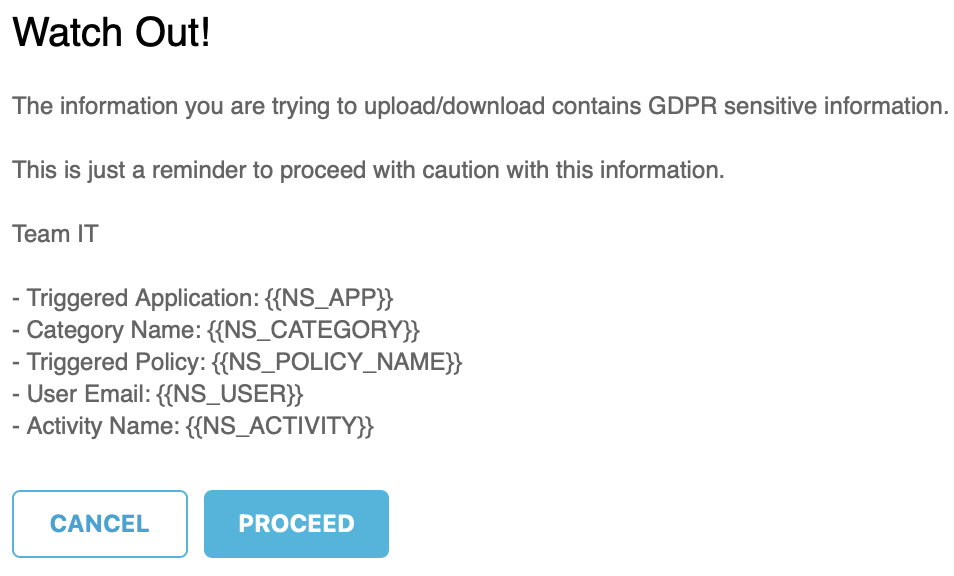
\includegraphics[scale=0.7]{user-warning.png}
    \caption[Netskope ZTNA pop-up notificatie]{Voorbeeld van een pop-up notificatie in Netskope ZTNA}
    \label{fig:user-alert}
\end{figure}

Deze gestroomlijnde workflow zorgt ervoor dat gebruikers slechts de toegang krijgen die ze nodig hebben (least privilege principe), terwijl de administratieve last wordt geminimaliseerd.

\subsection{Real-Time Protection Policies}

Een belangrijke component van de ZTNA-implementatie zijn de Real-Time Protection Policies die continu de toegang en het gebruik van applicaties monitoren en controleren:

\begin{itemize}
    \item \textbf{Applicatiespecifieke controle}: In tegenstelling tot traditionele VPN's wordt toegang verleend tot specifieke applicaties in plaats van het volledige netwerk, waardoor het aanvalsoppervlak aanzienlijk wordt verkleind.

    \item \textbf{Dynamische risicobeoordeling}: De policies evalueren voortdurend het risicoprofiel van de toegangssessie op basis van gebruikersgedrag, apparaatstatus en netwerkcontext. Deze dynamische evaluatie maakt real-time aanpassingen mogelijk indien het risicoprofiel verandert.

    \item \textbf{Granulaire CASB-integratie}: De combinatie van ZTNA met Cloud Access Security Broker (CASB) functionaliteit maakt het mogelijk om diepgaande controle toe te passen op gegevensstromen binnen applicaties, zoals het blokkeren van het uploaden van gevoelige informatie.

    \item \textbf{Continuous monitoring}: Zelfs na de initiële authenticatie blijft het systeem alle interacties monitoren op verdachte activiteiten of afwijkend gedrag, wat kan leiden tot onmiddellijke aanpassing van toegangsrechten of zelfs het verbreken van de sessie.
\end{itemize}

\subsection{Voordelen voor het bedrijf}
De implementatie van Netskope ZTNA met Okta-integratie biedt het bedrijf verschillende belangrijke voordelen~\autocite{Okta2025}:

\begin{itemize}
    \item \textbf{Vereenvoudigde toegang}: Medewerkers ervaren een consistente en gebruiksvriendelijke inlogprocedure voor alle applicaties, ongeacht hun locatie
    \item \textbf{Verhoogde beveiliging}: Het Zero Trust-model verkleint het aanvalsoppervlak en minimaliseert de impact van een potentiële inbreuk
    \item \textbf{Operationele efficiëntie}: Geautomatiseerde groep-gebaseerde configuratie vermindert de administratieve last en het risico op menselijke fouten
    \item \textbf{Verbeterde compliance}: Gedetailleerde logging en controle van toegangsactiviteiten ondersteunt audit- en compliance-vereisten
    \item \textbf{Schaalbaarheid}: Het model schaalt moeiteloos mee met veranderingen in de organisatie, zowel in grootte als structuur
\end{itemize}

Door Netskope ZTNA te implementeren met Okta wordt een belangrijke stap gezet in de transformatie naar een moderne, secure-by-design infrastructuur die medewerkers flexibiliteit biedt zonder onder te hoeven doen aan beveiliging.

\subsection{Bedrijfsapplicaties beveiligen via Okta en Netskope egress IP's}

Een cruciaal onderdeel van de ZTNA-implementatie binnen Netskope is de beveiliging van bedrijfsapplicaties via Okta, waarbij toegang wordt beperkt tot uitsluitend verkeer dat via de Netskope Security Cloud verloopt. Deze aanpak vormt een effectieve extra beveiligingslaag die voorkomt dat gebruikers de Netskope-client kunnen omzeilen, en tevens verzekert dat alle toegang tot bedrijfsapplicaties onderworpen wordt aan de volledige reeks beveiligingscontroles~\autocite{Okta2025-2}.

\vspace{2ex}

De beveiliging van bedrijfsapplicaties via Okta en Netskope egress IP's werkt volgens het volgende principe:

\begin{enumerate}
    \item \textbf{Netskope egress IP's identificeren}: Elke Netskope Security Cloud POP (Point of Presence) heeft specifieke egress IP-adressen waarvanuit verkeer de Netskope-cloud verlaat richting de doelwebsites en -applicaties. Voor de BE-BRU1 POP, die in onze implementatie wordt gebruikt, zijn deze egress IP's gedocumenteerd en relatief statisch.

    \item \textbf{Okta configureren}: Binnen de Okta-administratie worden de toegangsbeleiden voor bedrijfsapplicaties zodanig geconfigureerd dat ze alleen toegang toestaan vanaf de geautoriseerde Netskope egress IP-adressen. Dit gebeurt via de Network Zones functionaliteit in Okta.

    \item \textbf{Geforceerde routering}: Door deze configuratie wordt alle toegang tot de bedrijfsapplicaties geforceerd via de Netskope Security Cloud, omdat alleen verkeer afkomstig van de Netskope egress IP's wordt toegestaan door Okta.
\end{enumerate}

Als een medewerker op zijn Okta dashboard zit en Netskope staat niet aan, dan krijgt men een melding te zien als in Figuur \ref{fig:okta-denied}. Deze zal worden getoond op applicaties waarvoor Netskope ingeschakeld moet zijn.
\begin{figure}[H]
    \centering
    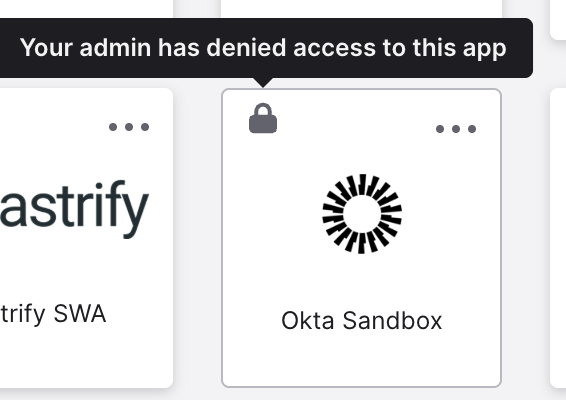
\includegraphics[scale=0.3]{okta-denied.png}
    \caption[Geen Netskope Okta melding]{Voorbeeld van een melding in Okta wanneer Netskope niet is ingeschakeld}
    \label{fig:okta-denied}
\end{figure}

\subsection{Voordelen voor beveiliging}

Deze integratie biedt verschillende belangrijke beveiligingsvoordelen:

\begin{itemize}
    \item \textbf{Volledige inspectie}: Al het verkeer naar bedrijfsapplicaties doorloopt de Netskope beveiligingscontroles, inclusief DLP, malware-scanning en policy enforcement
    \item \textbf{Omzeiling preventie}: Gebruikers kunnen niet bewust of onbewust de beveiligingsmaatregelen omzeilen, wat een belangrijke bescherming biedt tegen shadow IT
    \item \textbf{Contextbewuste toegang}: Netskope kan rijke contextinformatie toevoegen aan de toegangsbesluiten, zoals apparaatgezondheid, gebruikerslocatie en risicobeoordelingen
    \item \textbf{Gecentraliseerde logging}: Alle toegangspogingen worden uniform gelogd binnen het Netskope platform, wat beveiligingsanalyse en incident response verbetert
\end{itemize}

Door bedrijfsapplicaties te beveiligen via Okta en Netskope egress IP's, wordt een belangrijk onderdeel van de ZTNA-architectuur geïmplementeerd dat helpt bij het realiseren van een consistent Zero Trust-model. Waarbij alle toegang wordt geverifieerd, geautoriseerd en gecontroleerd, ongeacht de locatie van de gebruiker of het netwerk waarmee zij verbinding maken.

\section{Netskope Publisher}

De Netskope Publisher vormt een essentiële component binnen de SASE-architectuur door een secure gateway te bieden tussen het Netskope Security Cloud platform en private applicaties in het bedrijfsnetwerk. Anders dan de Netskope Client, die op eindpunten wordt geïnstalleerd, wordt de Publisher geplaatst binnen de netwerkinfrastructuur om private applicaties veilig toegankelijk te maken voor geauthenticeerde gebruikers.

\subsection{Werkingsprincipe van de Netskope Publisher}

De Publisher functioneert volgens een specifiek mechanisme dat de veiligheid van applicatietoegang garandeert~\autocite{Netskope2025-6}:

\begin{enumerate}
    \item De Publisher wordt uitgerold in het netwerksegment waar de applicatieresources zich bevinden. Dit kan een datacenter, cloud-omgeving of een ander netwerkgebied zijn waar private applicaties worden gehost.

    \item Bij opstart registreert de Publisher zich bij de Netskope Security Cloud en authenticeert zichzelf via certificaatauthenticatie, waarbij een beveiligde TLS-tunnel wordt opgebouwd tussen de Publisher en het Netskope-platform.

    \item Wanneer een gebruiker toegang vraagt tot een private applicatie, wordt het verzoek eerst door de Netskope Cloud gevalideerd volgens het bestaande beveiligingsbeleid, inclusief gebruikersidentiteit, apparaatverificatie en contextfactoren.

    \item Bij goedkeuring wordt het verzoek via de beveiligde tunnel doorgestuurd naar de Publisher, die het vervolgens naar de juiste applicatieresource routeert, waarmee een beveiligde end-to-end verbinding tot stand wordt gebracht.
\end{enumerate}

Deze architectuur zorgt ervoor dat private applicaties onzichtbaar blijven voor ongeautoriseerde gebruikers, terwijl ze volledig toegankelijk zijn voor geautoriseerde medewerkers, ongeacht hun locatie of het netwerk van waaruit ze verbinding maken.

\subsection{Implementatie in de proof of concept}

Voor onze proof of concept hebben we de Publisher geïmplementeerd in de GCP region waar de private applicaties worden gehost.

\vspace{2ex}

De implementatie van de Netskope Publisher binnen onze SASE-architectuur heeft geleid tot een aanzienlijke verbetering in zowel de beveiligingsposture als de gebruikerservaring, waarbij medewerkers nu veilig toegang hebben tot bedrijfsapplicaties vanuit elke locatie, zonder de overhead en beperkingen van traditionele VPN-oplossingen.

\section{Netskope Dashboard}
Voor de proof of concept is een Netskope Advanced Analytics dashboard (zie Figuur \ref{fig:dashboard-1}) opgezet om het netwerkverkeer en de beveiliging binnen het bedrijf overzichtelijk op te volgen. Dit dashboard geeft het Team IT in één oogopslag inzicht in wat er gebeurt binnen de Netskope-omgeving, zowel op het vlak van gebruikersacties als beveiligingsincidenten.

\subsection{Dashboard functionaliteiten}
Het dashboard toont onder andere:
\begin{itemize}
    \item \textbf{Device Overview}: Op Figuur \ref{fig:dashboard-1} wordt een overzicht gegeven van alle apparaten die wel of geen verbinding hebben met de Netskope Security Cloud. Hier kan men ook zien bij hoeveel apparaten private access of internet security is ingeschakeld. Ook wordt er weergegeven hoeveel gebruikers manueel hun Netskope hebben uitgeschakeld.
    \item \textbf{Malware}: Op Figuur \ref{fig:dashboard-1} wordt weergegeven welke malware er is gedetecteerd en de specifieke details van deze malware. Ook worden malsites weergegeven, dit zijn websites die gebruikt worden om malware te verspreiden. Uiteindelijk wordt er een trendlijn weergegeven van de aantal malware en malsites detecties over de gekozen periode.
    \item \textbf{User Behavior Analytics (UBA)}: Op Figuur \ref{fig:dashboard-2} wordt een grote flow matrix weergegeven van alle gedetecteerde gebruikersactiviteiten. Deze flows worden geleid naar het platform waar deze activiteiten zijn gedetecteerd.
    \item \textbf{AI Usage}: Op Figuur \ref{fig:dashboard-3} wordt een overzicht weergegeven van het AI-gebruik binnen het bedrijf. Er wordt getoond hoeveel gebruikers AI gebruiken en welke AI services worden gebruikt. Verder wordt er getoond wat de grootste services zijn en welke gevolgen deze hebben gegeven, dit kan gaan van een user coaching die wordt gegeven of een allow. Binnen de user coaching wordt er dan ook getoond welke actie de gebruiker heeft genomen.
\end{itemize}

\begin{figure}[H]
    \centering
    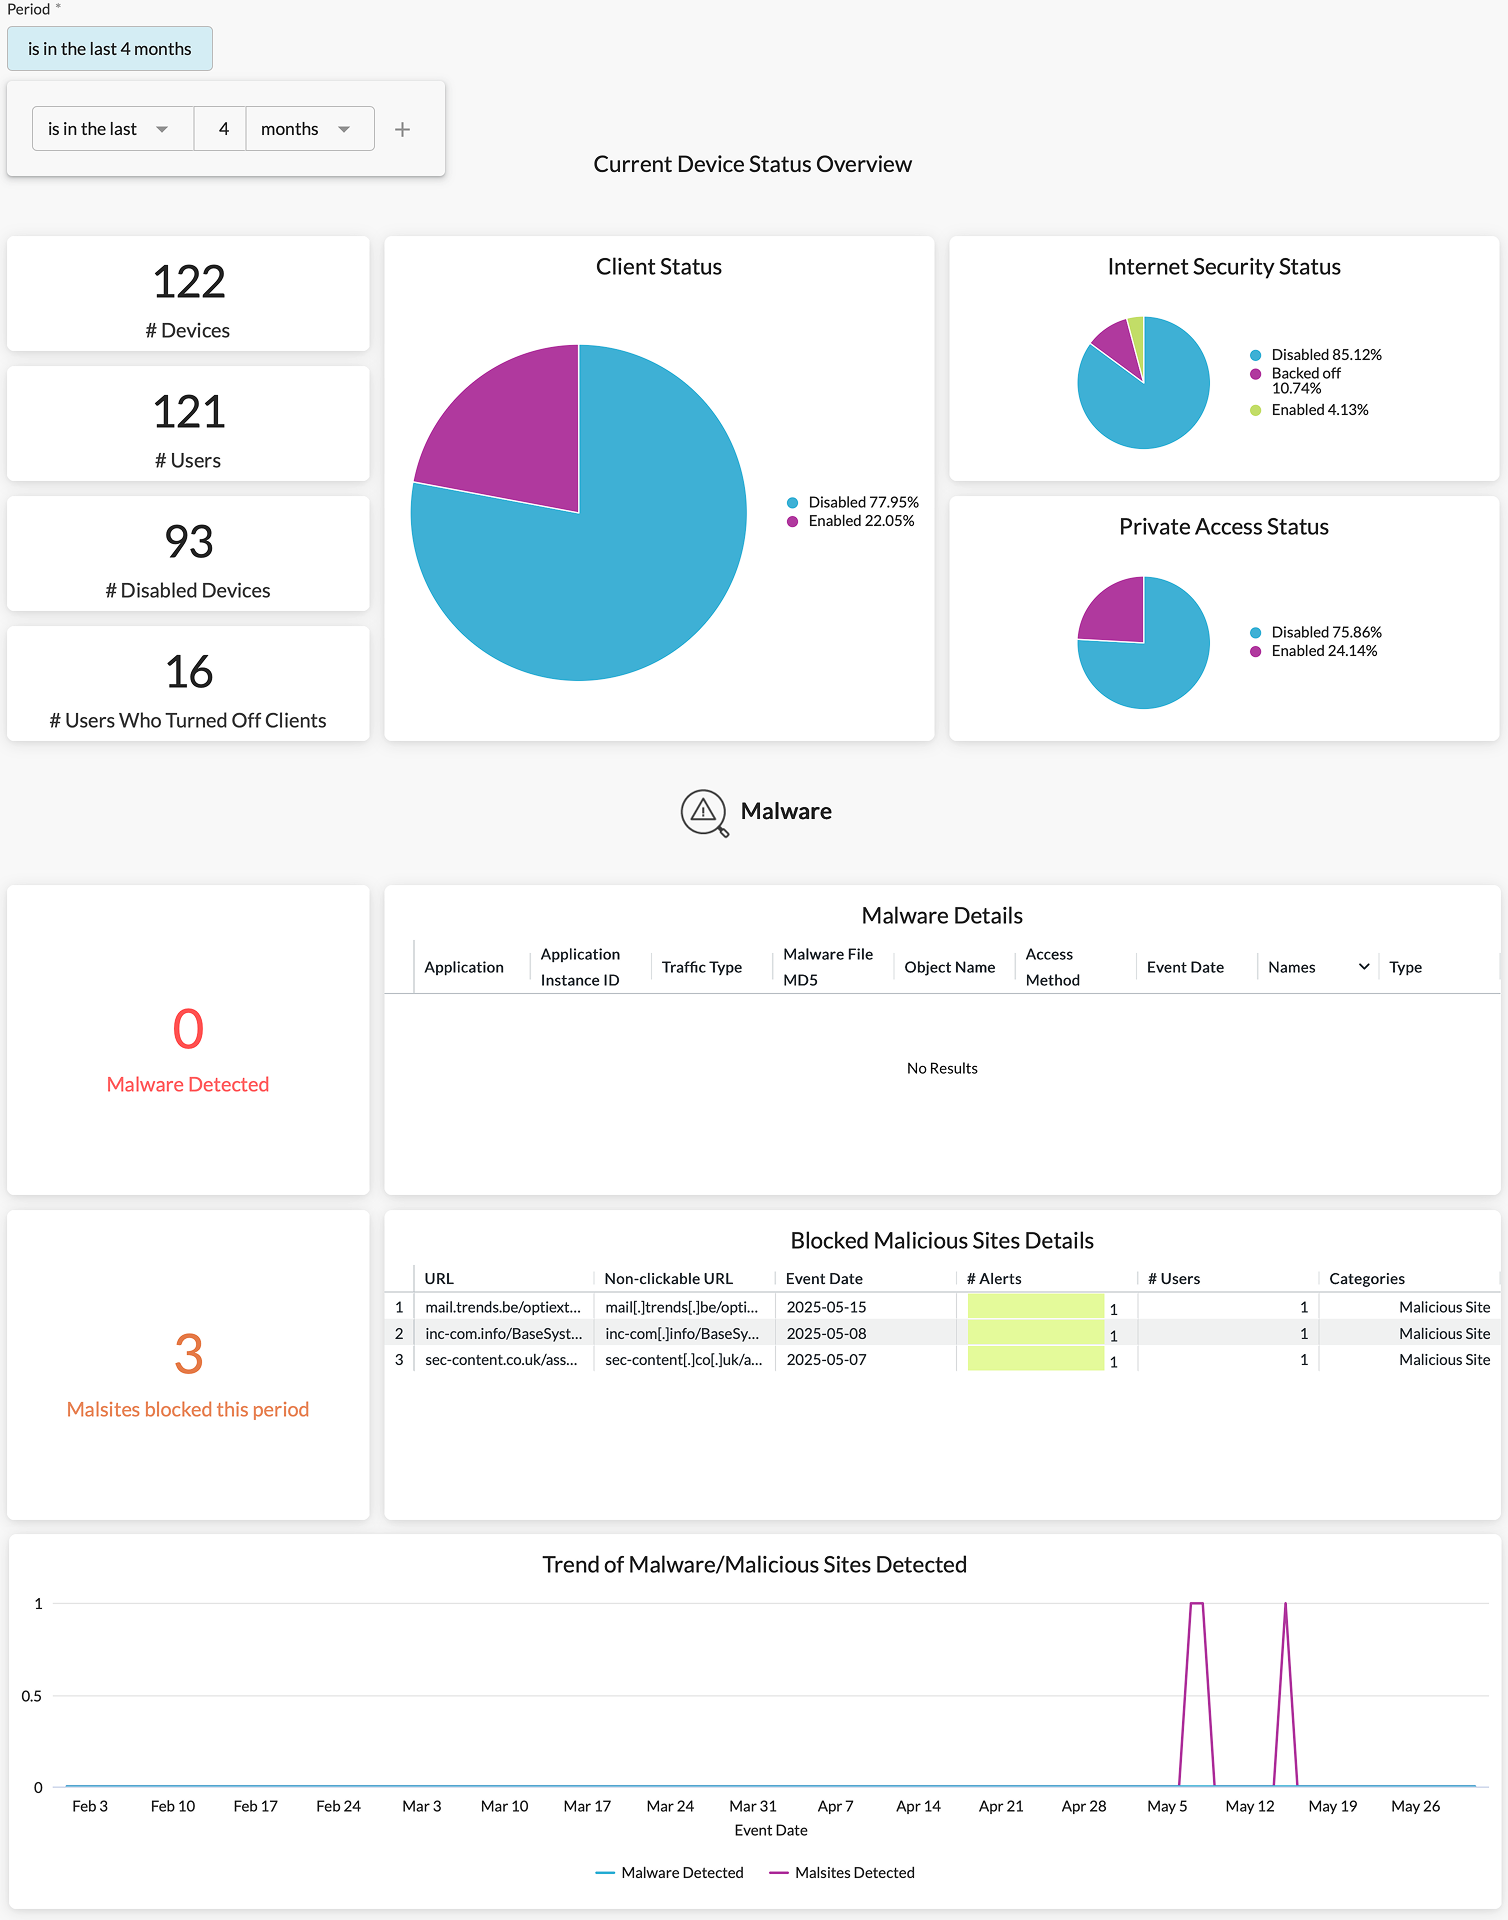
\includegraphics[width=\textwidth]{dashboard-1.png}
    \caption[Netskope Advanced Analytics dashboard - Deel 1]{Eerste deel van het Netskope Advanced Analytics dashboard}
    \label{fig:dashboard-1}
\end{figure}
\begin{figure}[H]
    \centering
    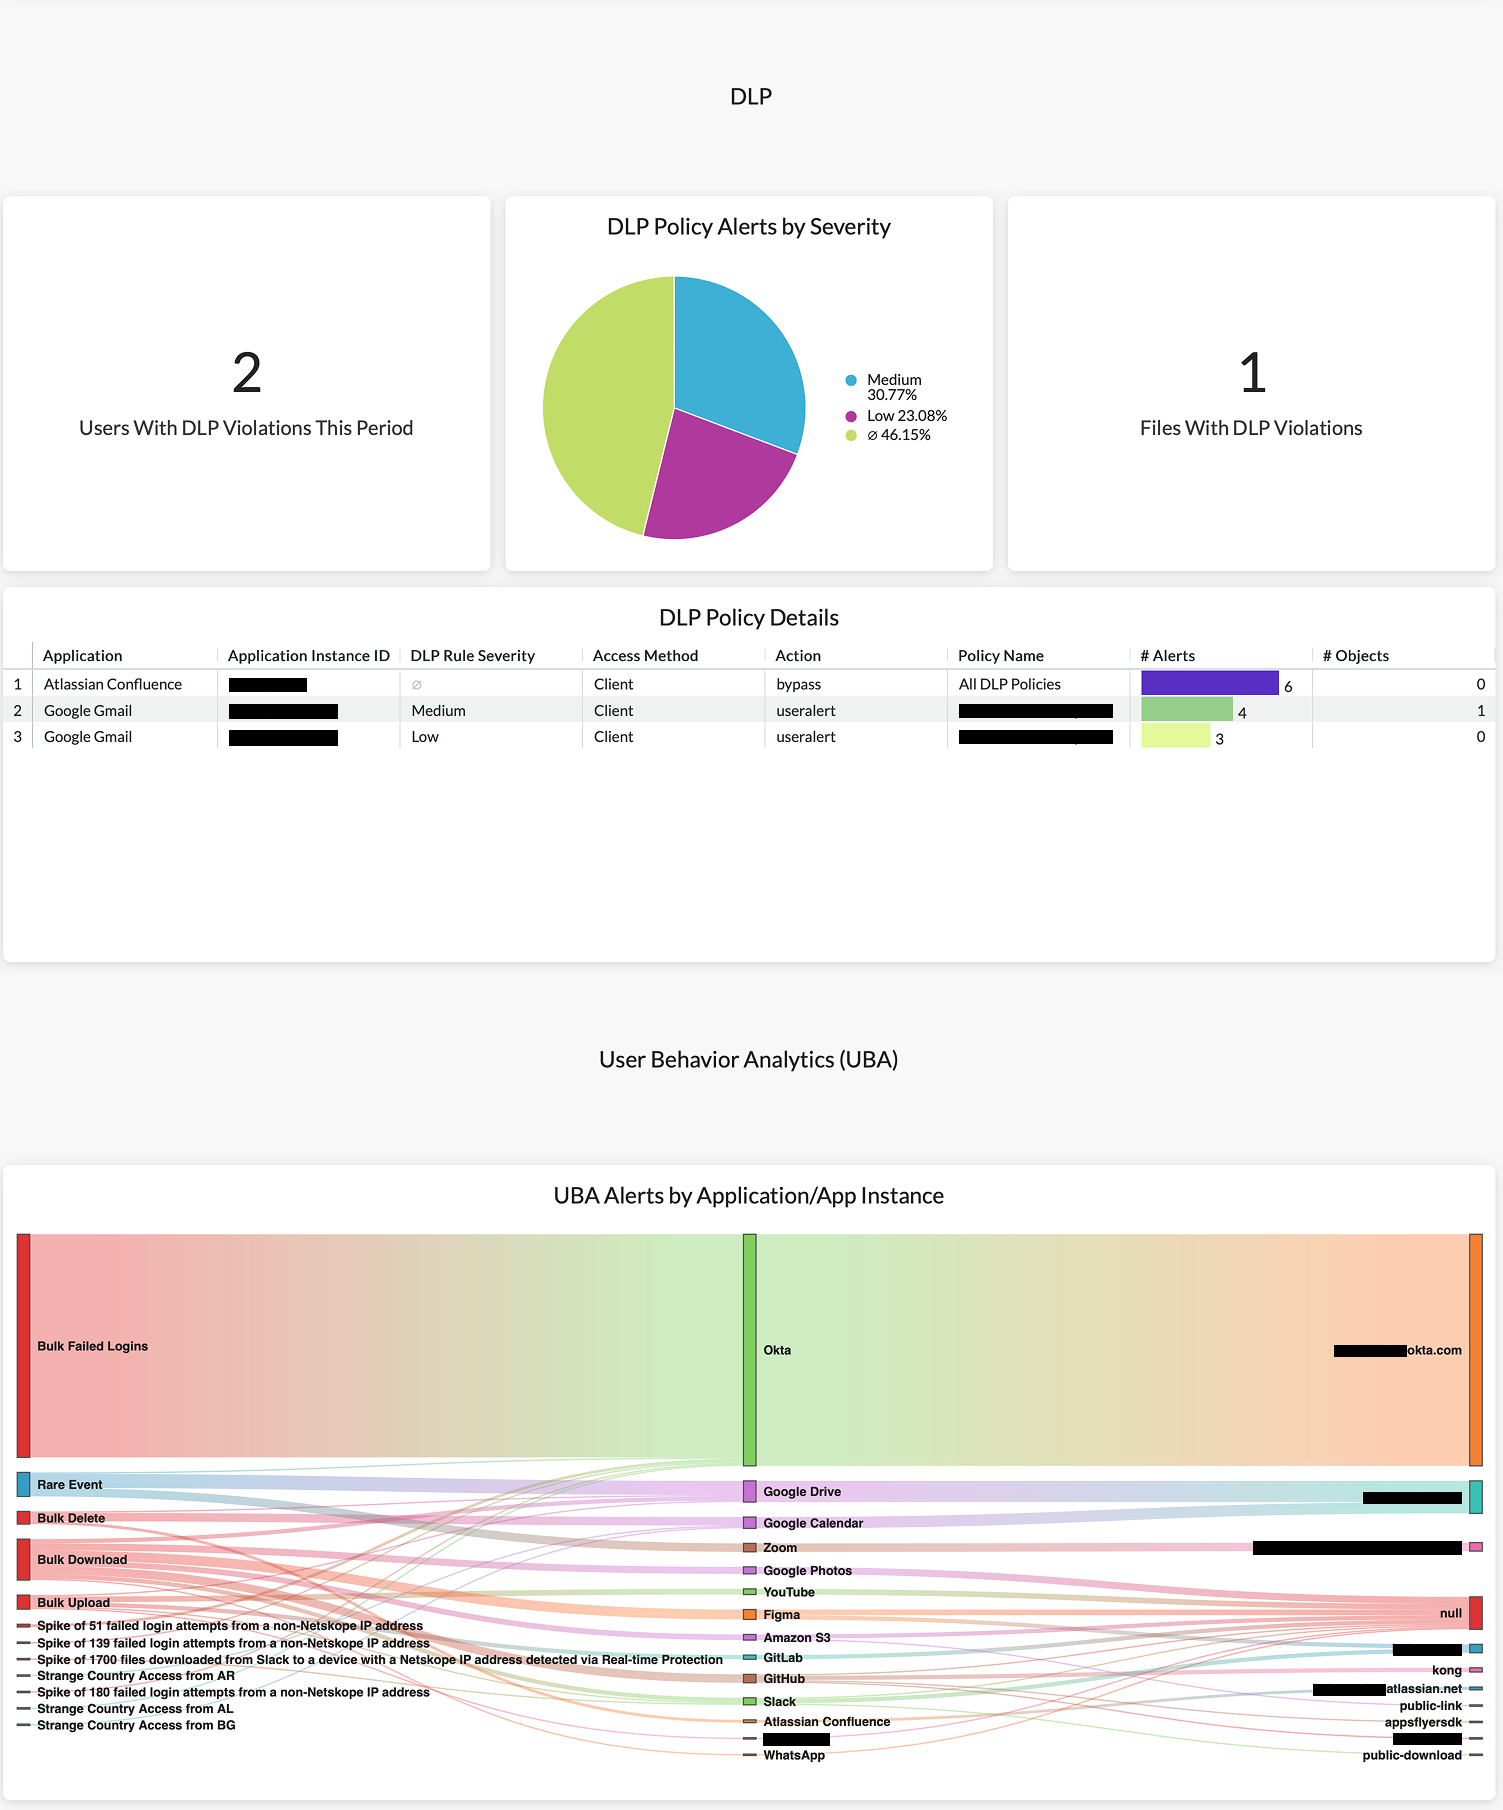
\includegraphics[width=\textwidth]{dashboard-2.png}
    \caption[Netskope Advanced Analytics dashboard - Deel 2]{Tweede deel van het Netskope Advanced Analytics dashboard}
    \label{fig:dashboard-2}
\end{figure}
\begin{figure}[H]
    \centering
    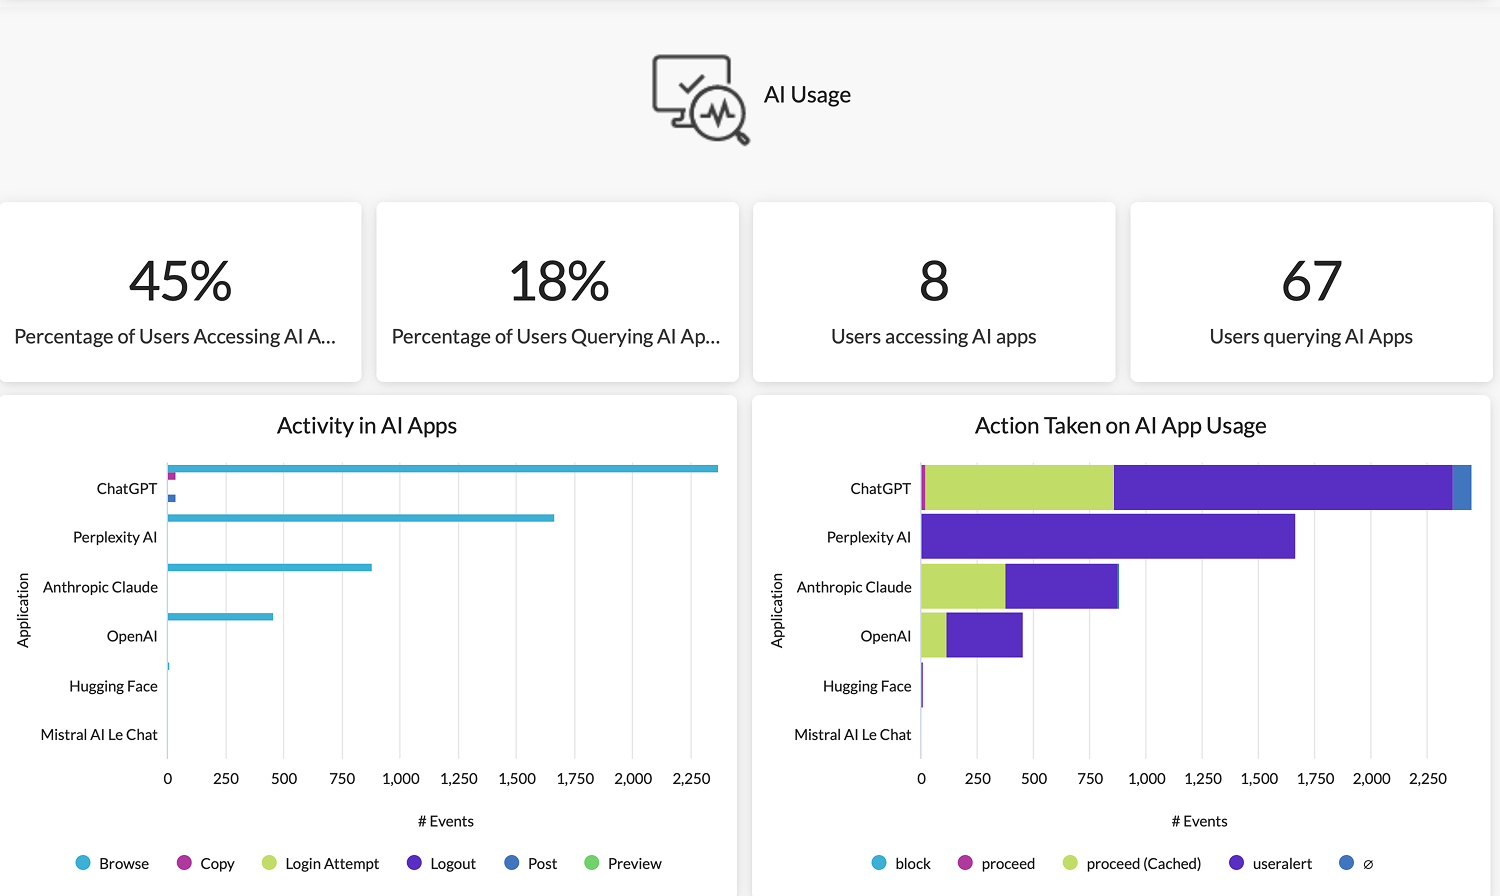
\includegraphics[width=\textwidth]{dashboard-3.png}
    \caption[Netskope Advanced Analytics dashboard - Deel 3]{Derde deel van het Netskope Advanced Analytics dashboard}
    \label{fig:dashboard-3}
\end{figure}

Het dashboard wordt dagelijks gebruikt om trends te volgen, incidenten te onderzoeken en het beleid waar nodig aan te passen. Zo kan het team bijvoorbeeld bij een toename van geblokkeerde uploads naar Google Drive nagaan of de policy moet worden aangepast of dat er extra uitleg aan gebruikers nodig is.

\vspace{2ex}

Door deze inzichten kan het bedrijf sneller reageren op problemen en blijft de controle over de beveiliging en het gebruik van cloudapplicaties behouden. Het dashboard zorgt voor meer overzicht, snellere detectie van problemen en maakt het makkelijker om de Netskope-omgeving goed te beheren. Het helpt het Team IT om beter onderbouwde beslissingen te nemen en de beveiliging continu te verbeteren.

\vspace{2ex}

Het dashboard wordt wekelijks overgebracht aan het Team IT via mail. Dit zorgt ervoor dat het team altijd op de hoogte is van de laatste ontwikkelingen en trends binnen de Netskope-omgeving, en stelt hen in staat om proactief te reageren op eventuele problemen of veranderingen.

%%=============================================================================
%% Conclusie
%%=============================================================================

\chapter{Conclusie}%
\label{ch:conclusie}

% TODO: Trek een duidelijke conclusie, in de vorm van een antwoord op de
% onderzoeksvra(a)g(en). Wat was jouw bijdrage aan het onderzoeksdomein en
% hoe biedt dit meerwaarde aan het vakgebied/doelgroep? 
% Reflecteer kritisch over het resultaat. In Engelse teksten wordt deze sectie
% ``Discussion'' genoemd. Had je deze uitkomst verwacht? Zijn er zaken die nog
% niet duidelijk zijn?
% Heeft het onderzoek geleid tot nieuwe vragen die uitnodigen tot verder 
%onderzoek?

\section{Beantwoording van de onderzoeksvraag}

De centrale onderzoeksvraag "Hoe kan een SASE-architectuur worden geïmplementeerd binnen de hybride cloudomgeving van een softwarebedrijf gebruikmakend van het Netskope platform?" kan op basis van dit onderzoek en de gemeten resultaten positief worden beantwoord. Het ontwikkelde proof of concept toont concrete en meetbare resultaten die de effectiviteit van de SASE-implementatie valideren.

\vspace{2ex}

De implementatie heeft aangetoond dat de geïdentificeerde netwerk- en security-uitdagingen in de hybride cloudomgeving effectief kunnen worden aangepakt. De traditionele perimetergebaseerde beveiligingsaanpak, die onvoldoende veiligheid en flexibiliteit bood, is vervangen door een Zero Trust-model dat contextbewuste beveiliging realiseert ongeacht gebruikerslocatie of apparaattype. De intelligente traffic steering op basis van gebruikerslocatie, gecombineerd met Okta-integratie voor identiteitsbeheer, zorgt voor een optimale balans tussen beveiliging, gebruikerservaring en prestaties.

\section{Bijdrage aan het onderzoeksdomein}

Dit onderzoek levert een concrete bijdrage aan het domein van SASE-implementaties door het ontwikkelen van een praktische implementatiemethodologie specifiek voor software agency bedrijven. De vierfasenaanpak, literatuuronderzoek, requirements analyse, proof of concept ontwikkeling en validatie, biedt een herhaalbaar framework voor vergelijkbare implementaties.

\section{Meerwaarde voor het vakgebied en doelgroep}

Voor IT-professionals en bedrijven biedt dit onderzoek directe meerwaarde, door het demonstreren van een schaalbare beveiligingsarchitectuur die voldoet aan moderne compliance-eisen zonder de operationele flexibiliteit te beperken. De proof of concept toont aan dat SASE-implementaties niet alleen theoretisch haalbaar zijn, maar ook praktisch realiseerbaar binnen bestaande infrastructuren.

\vspace{2ex}

De integratie met populaire enterprise-tools zoals Okta voor identiteitsbeheer en Jamf voor device management illustreert hoe SASE naadloos kan worden geïntegreerd in bestaande IT-ecosystemen. Dit vermindert de implementatierisico's en verlaagt de drempel voor adoptie door andere organisaties in de sector.

\section{Kritische reflectie op het resultaat}

De resultaten die in Hoofdstuk \ref{ch:resultaten} worden samengevat, waren grotendeels conform de verwachtingen, hoewel enkele aspecten positiever uitvielen dan initieel voorzien. 

\vspace{2ex}

De gebruikersacceptatie van de Netskope Client bleek lager dan verwacht, desondanks de transparante communicatiestrategie en de minimale impact op de dagelijkse workflow. 

\vspace{2ex}

De intelligente traffic steering functionaliteit presteerde beter dan geanticipeerd, met nauwelijks merkbare latentieverschillen voor eindgebruikers. Toch waren de eindgebruikers aanvankelijk terughoudend om de nieuwe client te accepteren, wat wijst op de noodzaak van voortdurende change management inspanningen en training.

\vspace{2ex}

Een positief resultaat was de rijkdom aan analytische gegevens die het Netskope platform genereert. Het Advanced Analytics dashboard biedt inzichten die verder gaan dan louter beveiligingsmonitoring en ook waardevolle business intelligence leveren over applicatiegebruik en gebruikersgedrag.

\vspace{2ex}

Een onverwacht technisch probleem was de SSL certificaat interferentie met CLI tools, waarbij applicaties Netskope's SSL Inspection functionaliteit interpreteerden als potentiële Man-in-the-Middle attacks. Dit probleem werd succesvol opgelost door application-specific bypasses en selective SSL inspection policies, maar onderstreept het belang van uitgebreide applicatie-inventarisatie.

\section{Beperkingen en vervolgonderzoek}

Een belangrijke beperking van dit onderzoek is de beperkte onderzoeksperiode van 14 weken, wat de mogelijkheid om langetermijneffecten en gebruikersadoptie over meerdere maanden te evalueren niet mogelijk maakt. Een langdurig onderzoek zou meer inzicht kunnen geven in de evolutie van gebruikersgedrag en de optimalisatie van security policies over tijd.

\section{Conclusie}

Deze bachelorproef demonstreert dat SASE-architectuur via Netskope een praktisch haalbare oplossing biedt voor moderne hybride cloudomgevingen. De combinatie van company-wide Private Access implementatie (122 apparaten under management) met een testgroep van SWG/CASB functionaliteiten toont een effectieve implementatiestrategie die risico's mitigeert terwijl schaalbaarheid wordt gevalideerd.

\vspace{2ex}

De gemeten resultaten van 3 geblokkeerde malicious sites tot 2.100+ AI-events bij ChatGPT, illustreren niet alleen traditionele beveiligingsvoordelen, maar genereren ook unexpected business intelligence die verder gaat dan conventionele security monitoring. Deze concrete cijfers en inzichten vormen een solide basis voor de aanbeveling tot volledige productie-implementatie van alle SASE-componenten binnen software agency bedrijven.

\section{Onverwachte uitdagingen}
\subsection{Eindgebruikers}
Een van de grootste uitdagingen die ik niet had voorzien was het change management-aspect van de implementatie. Technisch gezien verliep de configuratie van Netskope vrij vlot, maar het overtuigen van eindgebruikers van de voordelen en het wegnemen van privacy-zorgen bleek veel complexer dan verwacht. Dit heeft mij geleerd dat succesvolle IT-implementaties evenveel over menselijke factoren gaan als over technologische.

\subsection{SSL certificaat}
Tijdens de implementatie van de Netskope SASE-architectuur ontstond een onverwacht technisch probleem waarbij verschillende applicaties, voornamelijk Command Line Interface (CLI) tools, faalden in hun normale werking. Deze applicaties genereerden SSL/TLS-gerelateerde fouten en weigerden verbindingen tot stand te brengen met externe services.

\vspace{2ex}

Het probleem werd veroorzaakt door Netskope's SSL Inspection functionaliteit, waarbij de Netskope Client een eigen SSL certificaat plaatst op uitgaande HTTPS-pakketten als onderdeel van de Next Gen Secure Web Gateway (SWG) inspectie. Deze techniek, bekend als SSL decryption, stelt de SASE-oplossing in staat om versleuteld verkeer te inspecteren op malware, data loss prevention (DLP) violations, en policy enforcement.

\vspace{2ex}

CLI tools en verschillende enterprise applicaties interpreteren deze certificaat-substitutie als een potentiële Man-in-the-Middle (MiTM) attack, wat resulteert in:

\begin{itemize}
    \item \textbf{Certificate Pinning violations}: Applicaties die specifieke certificaten verwachten van bekende services
    \item \textbf{Trust store conflicts}: Tools die hun eigen certificaat stores hanteren en geen system-wide certificaat updates accepteren
    \item \textbf{API connectivity failures}: RESTful API clients die strikte SSL verificatie hanteren
    \item \textbf{Package managers}: Tools zoals npm, pip, en apt die beveiligde repositories benaderen
\end{itemize}

\section{Persoonlijke reflectie}
\subsection{Leercurve}
Dit onderzoek heeft mijn begrip van moderne netwerkbeveiliging compleet veranderd. Toen ik begon met dit project, was mijn kennis van Zero Trust en SASE-architecturen grotendeels onbestaand. Het praktisch implementeren van een volledige Netskope-omgeving heeft mij echter doen inzien hoe complex en veelomvattend deze transformatie werkelijk is. De overgang van perimetergebaseerde beveiliging naar een Zero Trust-model vereist niet alleen technische aanpassingen, maar vraagt ook om een complete herziening van hoe organisaties over beveiliging denken. Het vraagt ook een enorme inspanning om de werknemers achter de nieuwe technologie te krijgen, dit was een van de grootste uitdagingen die ik tegenkwam die ik niet had verwacht. Het heeft mij ook een eerste ervaring gegeven met een groot project in een bedrijfsomgeving, wat een waardevolle aanvulling is op mijn academische kennis.


%---------- Bijlagen -----------------------------------------------------------

\appendix

\chapter{Onderzoeksvoorstel}

Het onderwerp van deze bachelorproef is gebaseerd op een onderzoeksvoorstel dat vooraf werd beoordeeld door de promotor. Dat voorstel is opgenomen in deze bijlage.

%% TODO: 
%\section*{Samenvatting}

% Kopieer en plak hier de samenvatting (abstract) van je onderzoeksvoorstel.

% Verwijzing naar het bestand met de inhoud van het onderzoeksvoorstel
%---------- Inleiding ---------------------------------------------------------

% TODO: Is dit voorstel gebaseerd op een paper van Research Methods die je
% vorig jaar hebt ingediend? Heb je daarbij eventueel samengewerkt met een
% andere student?
% Zo ja, haal dan de tekst hieronder uit commentaar en pas aan.

%\paragraph{Opmerking}

% Dit voorstel is gebaseerd op het onderzoeksvoorstel dat werd geschreven in het
% kader van het vak Research Methods dat ik (vorig/dit) academiejaar heb
% uitgewerkt (met medesturent VOORNAAM NAAM als mede-auteur).
% 

\section{Inleiding}%
\label{sec:inleiding}

De IT-sector wordt steeds vaker geconfronteerd met complexe beveiligingsuitdagingen, ook in hybride cloudomgevingen. 
Traditionele netwerkbeveiligingsmodellen, die vertrouwen op perimeterbescherming (waarbij de beveiliging zich vooral richt op het bewaken van de netwerkgrenzen via firewalls en VPNs), zijn niet langer toereikend in een tijdperk waarin remote werken, multi-cloud gebruik en gevoelige data-uitwisseling standaard zijn. 
Zero Trust is een beveiligingsstrategie die steeds meer aandacht krijgt, omdat het uitgaat van het principe "never trust, always verify", en de toegang tot resources strikt beperkt op basis van identiteit en context.

Een software agency bedrijf gespecialiseerd in digitale producten, heeft gekozen voor Netskope als oplossing om een Zero Trust Netwerkarchitectuur en een least privileged access model te implementeren. 
Deze keuze voor Netskope als Security Service Edge (SSE) platform dient niet alleen om gevoelige klantendata beter te beschermen, maar ook om te voldoen aan moderne IT-veiligheidsstandaarden die passen bij hun rol als innovatief technologiebedrijf.
De primaire doelgroep van deze bachelorproef is het interne sysops-team van het bedrijf, dat verantwoordelijk is voor de infrastructuur en beveiliging van hun IT-systemen. 
Secundair is het onderzoek relevant voor IT-professionals die verantwoordelijk zijn voor de implementatie van Zero Trust in vergelijkbare omgevingen.

Hoewel het bedrijf geen acuut beveiligingsprobleem ervaart, willen zij anticiperen op toekomstige risico's en voldoen aan de best practices voor IT-beveiliging.
De vraag die centraal staat in dit onderzoek is: "Hoe kan een Zero Trust Netwerkarchitectuur en een least privileged access model worden geïmplementeerd binnen de hybride cloudomgeving van een software agency bedrijf gebruikmakend van het Netskope platform?"

Om deze hoofdvraag te beantwoorden, wordt het onderzoek opgedeeld in volgende deelvragen:
Probleemdomein:
\begin{itemize}
  \item Welke security-risico's bestaan er in de huidige IT-infrastructuur van het bedrijf die met Netskope's Zero Trust features aangepakt kunnen worden?
  \item Welke security gaps bestaan er in de huidige perimeter-based beveiliging die Netskope moet oplossen?
  \item Hoe verhouden de huidige beveiligingsmaatregelen zich tot de mogelijkheden die Netskope biedt?
\end{itemize}

Oplossingsdomein:
\begin{itemize}
  \item Welke Netskope componenten zijn essentieel voor een succesvolle Zero Trust implementatie?
  \item Hoe kan Netskope optimaal geconfigureerd worden voor de hybride cloudomgeving van het bedrijf?
  \item Hoe kan een least privileged access model worden geïmplementeerd via Netskope's policy engine?
  \item Welke integraties tussen Netskope en bestaande systemen zijn nodig?
  \item Hoe kan de effectiviteit van de Netskope implementatie worden gevalideerd?
\end{itemize}

Het doel van deze bachelorproef is om een praktische invulling te geven aan Zero Trust binnen een software agency bedrijf. Om deze deelvragen te beantwoorden richt het onderzoek zich op drie hoofdaspecten:
\begin{itemize}
  \item Een grondige analyse van de huidige IT-omgeving bij het bedrijf en de bijhorende security-risico's.
  \item Het identificeren van essentiële Netskope componenten en configuraties die aansluiten bij de specifieke context van het bedrijf.
  \item Het ontwerpen en implementeren van een proof of concept die dient als blauwdruk voor toekomstige implementaties.
\end{itemize}

Een succesvol resultaat wordt behaald als er een concreet PoC wordt opgeleverd dat technisch functioneel is en aansluit bij de behoeften van het bedrijf, samen met een rapport waarin aanbevelingen worden gedaan voor de schaalbare implementatie van Zero Trust met Netskope.

%---------- Stand van zaken ---------------------------------------------------
% Hier beschrijf je de \emph{state-of-the-art} rondom je gekozen onderzoeksdomein, d.w.z.\ een inleidende, doorlopende tekst over het onderzoeksdomein van je bachelorproef. Je steunt daarbij heel sterk op de professionele \emph{vakliteratuur}, en niet zozeer op populariserende teksten voor een breed publiek. Wat is de huidige stand van zaken in dit domein, en wat zijn nog eventuele open vragen (die misschien de aanleiding waren tot je onderzoeksvraag!)?

% Je mag de titel van deze sectie ook aanpassen (literatuurstudie, stand van zaken, enz.). Zijn er al gelijkaardige onderzoeken gevoerd? Wat concluderen ze? Wat is het verschil met jouw onderzoek?

% Verwijs bij elke introductie van een term of bewering over het domein naar de vakliteratuur, bijvoorbeeld~\autocite{Hykes2013}! Denk zeker goed na welke werken je refereert en waarom.

%Draag zorg voor correcte literatuurverwijzingen! Een bronvermelding hoort thuis \emph{binnen} de zin waar je je op die bron baseert, dus niet er buiten! Maak meteen een verwijzing als je gebruik maakt van een bron. Doe dit dus \emph{niet} aan het einde van een lange paragraaf. Baseer nooit teveel aansluitende tekst op eenzelfde bron.

% Als je informatie over bronnen verzamelt in JabRef, zorg er dan voor dat alle nodige info aanwezig is om de bron terug te vinden (zoals uitvoerig besproken in de lessen Research Methods).

\section{Literatuurstudie}%
\label{sec:literatuurstudie}

Zero Trust is een steeds belangrijker wordend model voor netwerkbeveiliging, vooral in omgevingen waar gevoelige data verwerkt wordt. 
Het model is gebaseerd op de stelling dat geen enkel apparaat, gebruiker of systeem automatisch te vertrouwen is, zelfs niet als deze zich binnen het netwerk bevinden. 
De nadruk ligt op het continu verifiëren van gebruikersidentiteit, het beperken van toegang tot strikt noodzakelijke bronnen (least privileged access), en het monitoren van netwerkactiviteiten om verdachte handelingen snel te identificeren en aan te pakken.

Netskope, het platform dat het bedrijf heeft gekozen voor hun Zero Trust implementatie, definieert Zero Trust als een beveiligingsmodel waarbij niemand blind vertrouwd wordt binnen het netwerk of toegang krijgt tot resources, applicaties of data totdat ze gevalideerd zijn als legitieme gebruiker met een legitieme behoefte~\autocite{Netskope2020}. Hun Security Service Edge (SSE) architectuur implementeert deze principes via een data-centrische aanpak gebaseerd op zes kernpijlers:

\begin{itemize}
  \item User \& Device: Authenticatie en autorisatie van gebruikers en apparaten
  \item Network \& Environment: Segmentatie en toegangscontrole op netwerkniveau
  \item Application \& Workload: Applicatie-specifieke toegangscontrole en monitoring
  \item Data: Databescherming en classificatie
  \item Visibility \& Analytics: Continue monitoring en gedragsanalyse
  \item Automation \& Orchestration: Geautomatiseerde response en integratie
\end{itemize}

Volgens Microsoft is de kern van het Zero Trust-model gebaseerd op drie belangrijke principes: altijd verifiëren, nooit vertrouwen; minimaal toegang verlenen; en schade beperken bij inbreuk. Dit houdt in dat de toegang tot systemen of data niet alleen wordt beperkt op basis van de locatie van de gebruiker of het apparaat, maar altijd afhangt van de identiteit, rol en andere specifieke toegangsbeperkingen~\autocite{Microsoft2024}. Netskope implementeert deze principes via een gelaagde aanpak met Policy Enforcement Points (PEPs) op drie niveaus:

\begin{itemize}
  \item Network/Resource PEP: Controleert netwerktoegang en basiscommunicatie
  \item Application PEP: Beheert toegang tot specifieke applicaties en workloads
  \item Data PEP: Zorgt voor databescherming en compliance
\end{itemize}

Kaspersky benadrukt het belang van de technologieën die Zero Trust mogelijk maken, zoals multi-factor authenticatie (MFA), versleuteling van communicatie en geavanceerde netwerkmonitoringtools~\autocite{Kaspersky2024}. Netskope's platform integreert deze technologieën in een uitgebreid security framework dat onder andere bestaat uit:

\begin{itemize}
  \item Device en user authenticatie via een client certificaat infrastructuur
  \item TLS-beveiligde tunneling voor alle communicatie
  \item Data Loss Prevention (DLP) met meer dan 3000 data identifiers en 1400 bestandstypes
  \item Machine learning-gebaseerde User and Entity Behavior Analytics (UEBA)
  \item Real-time threat protection met meer dan 40 threat intelligence feeds
\end{itemize}

De implementatie van Zero Trust vereist zorgvuldige planning, vooral in complexe netwerkomgevingen.

Uit onderzoek van MIT Lincoln Laboratory blijkt dat Zero Trust-architecturen bijzonder effectief zijn tegen insiderdreigingen, zoals misbruik van gecompromitteerde credentials of onbevoegde toegang door eigen medewerkers. 
Dit risico is relevant voor het onderzochte bedrijf, waar ontwikkelaars en externe partners toegang hebben tot gevoelige klantdata. 
MIT benadrukt dat een succesvolle Zero Trust-implementatie niet alleen technologische verandering vereist (zoals granular access control), maar ook organisatorische aanpassingen, zoals het trainen van medewerkers en het opstellen van duidelijk beleid voor toegangsverificatie. 
Dit sluit aan bij Netskope’s focus op User \& Device workflows en gedragsanalyse, waarbij continue verificatie van gebruikers en apparaten centraal staat. 
Tegelijkertijd waarschuwt MIT voor de complexiteit van hybride implementaties, waarbij on-premises systemen en clouddiensten geïntegreerd moeten worden—een uitdaging die het bedrijf direct ondervindt en waar Netskope’s SSE-platform een antwoord op biedt.~\autocite{MIT2022}

Netskope biedt hiervoor een gestructureerde aanpak met specifieke operationele workflows:

\begin{itemize}
  \item User/Device workflow voor initiële authenticatie en continue validatie
  \item Network/Resource workflow voor toegangscontrole en segmentatie
  \item Data Protection workflow voor databescherming en compliance
\end{itemize}

Deze workflows worden ondersteund door een automation engine die continue monitoring uitvoert op zeven dimensies van gebruikersactiviteit: tijd, dag, locatie, apparaat, service, activiteit en object. Dit zorgt voor een dynamische beveiligingsposture die zich aanpast aan veranderende omstandigheden en dreigingen~\autocite{Netskope2020}.

Deze literatuurstudie toont aan dat de keuze van het bedrijf voor Netskope aansluit bij moderne best practices voor Zero Trust implementatie. Het platform biedt niet alleen de technische capabilities voor robuuste beveiliging, maar ook de flexibiliteit en schaalbaarheid die nodig zijn voor een hybride cloudomgeving. De gelaagde aanpak met specifieke PEPs en geautomatiseerde workflows zorgt voor een balans tussen strikte beveiliging en operationele efficiëntie.
% Voor literatuurverwijzingen zijn er twee belangrijke commando's:
% \autocite{KEY} => (Auteur, jaartal) Gebruik dit als de naam van de auteur
%   geen onderdeel is van de zin.
% \textcite{KEY} => Auteur (jaartal)  Gebruik dit als de auteursnaam wel een
%   functie heeft in de zin (bv. ``Uit onderzoek door Doll & Hill (1954) bleek
%   ...'')

% Je mag deze sectie nog verder onderverdelen in subsecties als dit de structuur van de tekst kan verduidelijken.

%---------- Methodologie ------------------------------------------------------
% Hier beschrijf je hoe je van plan bent het onderzoek te voeren. Welke onderzoekstechniek ga je toepassen om elk van je onderzoeksvragen te beantwoorden? Gebruik je hiervoor literatuurstudie, interviews met belanghebbenden (bv.~voor requirements-analyse), experimenten, simulaties, vergelijkende studie, risico-analyse, PoC, \ldots?

%Valt je onderwerp onder één van de typische soorten bachelorproeven die besproken zijn in de lessen Research Methods (bv.\ vergelijkende studie of risico-analyse)? Zorg er dan ook voor dat we duidelijk de verschillende stappen terug vinden die we verwachten in dit soort onderzoek!

%Vermijd onderzoekstechnieken die geen objectieve, meetbare resultaten kunnen opleveren. Enquêtes, bijvoorbeeld, zijn voor een bachelorproef informatica meestal \textbf{niet geschikt}. De antwoorden zijn eerder meningen dan feiten en in de praktijk blijkt het ook bijzonder moeilijk om voldoende respondenten te vinden. Studenten die een enquête willen voeren, hebben meestal ook geen goede definitie van de populatie, waardoor ook niet kan aangetoond worden dat eventuele resultaten representatief zijn.

%Uit dit onderdeel moet duidelijk naar voor komen dat je bachelorproef ook technisch voldoen\-de diepgang zal bevatten. Het zou niet kloppen als een bachelorproef informatica ook door bv.\ een student marketing zou kunnen uitgevoerd worden.

%Je beschrijft ook al welke tools (hardware, software, diensten, \ldots) je denkt hiervoor te gebruiken of te ontwikkelen.

%Probeer ook een tijdschatting te maken. Hoe lang zal je met elke fase van je onderzoek bezig zijn en wat zijn de concrete \emph{deliverables} in elke fase?

\section{Methodologie}%
\label{sec:methodologie}

Dit onderzoek volgt een systematische aanpak die bestaat uit drie hoofdfasen: literatuuronderzoek, technische analyse, en proof of concept ontwikkeling. De totale onderzoeksduur bedraagt 14 weken.

\subsection{Fase 1: Literatuuronderzoek (3 weken)}
Deze fase richt zich op het verzamelen van theoretische kennis en best practices:
\begin{itemize}
  \item Week 1-2: 
  \begin{itemize}
    \item Analyse van Netskope's technische documentatie en architectuur
    \item Bestudering van Netskope's Zero Trust Reference Architecture
    \item Onderzoek naar best practices voor Netskope implementaties
  \end{itemize}
  \item Week 3: 
  \begin{itemize}
    \item Synthese van bevindingen
    \item Opstellen van Netskope-specifiek implementatieplan
  \end{itemize}
  \item Deliverable: Implementatieplan met Netskope configuratierichtlijnen
\end{itemize}

\subsection{Fase 2: Technische analyse (4 weken)}

\subsubsection{Security audit (2 weken)}
\begin{itemize}
  \item Week 1: 
  \begin{itemize}
    \item Analyse van huidige netwerkinfrastructuur voor Netskope integratie
    \item Inventarisatie van te beveiligen resources en applicaties
  \end{itemize}
  \item Week 2:
  \begin{itemize}
    \item Assessment van integratiepunten voor Netskope
    \item Identificatie van benodigde Policy Enforcement Points
  \end{itemize}
  \item Deliverable: Technisch rapport met integratievereisten
\end{itemize}

\subsubsection{Requirements analyse (2 weken)}
\begin{itemize}
  \item Analyse van gebruikersprofielen voor Netskope policies
  \item Identificatie van kritieke applicaties en data flows
  \item In kaart brengen van benodigde security policies
  \item Deliverable: Requirements document voor Netskope configuratie
\end{itemize}

\subsection{Fase 3: Proof of Concept (7 weken)}

\subsubsection{PoC Setup (4 weken)}
Ontwikkeling van testomgeving met Netskope componenten:

\begin{enumerate}
  \item Week 1-2: Basis infrastructuur
  \begin{itemize}
    \item Opzetten Netskope tenant
    \item Configuratie van Identity and Access Management
    \item Implementatie van Netskope client op test endpoints
  \end{itemize}

  \item Week 3-4: Policy en Security configuratie
  \begin{itemize}
    \item Configuratie van Resource, Application en Data PEPs
    \item Implementatie van security policies
    \item Setup van monitoring en logging
  \end{itemize}
  \item Deliverable: Functionele Netskope PoC omgeving
\end{enumerate}

\subsubsection{PoC Validatie (3 weken)}
\begin{itemize}
  \item Week 1: Security testing
  \begin{itemize}
    \item Validatie van Zero Trust policies
    \item Testing van MFA en toegangscontrole
    \item DLP functionaliteit verificatie
    \item Testing van dynamische toegangscontrole (‘trip wires’)
  \end{itemize}
  
  \item Week 2: Performance testing
  \begin{itemize}
    \item Latency metingen van Netskope security cloud
    \item End-user experience validatie
    \item Resource impact analyse
  \end{itemize}
  
  \item Week 3: Documentatie
  \begin{itemize}
    \item Opstellen van implementatiehandleiding
    \item Documenteren van best practices
    \item Voorbereiden eindrapportage
  \end{itemize}
  \item Deliverable: Validatierapport en implementatiedocumentatie
\end{itemize}

Deze methodologie is specifiek afgestemd op de implementatie van Zero Trust via het Netskope platform, waarbij elke fase concrete technische deliverables oplevert. De focus ligt op het correct configureren en valideren van Netskope's security features, met voldoende tijd voor iteratie en optimalisatie van de implementatie.

%---------- Verwachte resultaten ----------------------------------------------
%Hier beschrijf je welke resultaten je verwacht. Als je metingen en simulaties uitvoert, kan je hier al mock-ups maken van de grafieken samen met de verwachte conclusies. Benoem zeker al je assen en de onderdelen van de grafiek die je gaat gebruiken. Dit zorgt ervoor dat je concreet weet welk soort data je moet verzamelen en hoe je die moet meten.

%Wat heeft de doelgroep van je onderzoek aan het resultaat? Op welke manier zorgt jouw bachelorproef voor een meerwaarde?

%Hier beschrijf je wat je verwacht uit je onderzoek, met de motivatie waarom. Het is \textbf{niet} erg indien uit je onderzoek andere resultaten en conclusies vloeien dan dat je hier beschrijft: het is dan juist interessant om te onderzoeken waarom jouw hypothesen niet overeenkomen met de resultaten.

\section{Verwacht resultaat, conclusie}%
\label{sec:verwachte_resultaten}

Het belangrijkste verwachte resultaat is het succesvol opzetten van een Proof of Concept (PoC) die demonstreert hoe Netskope's Zero Trust architectuur effectief kan worden geïmplementeerd binnen de bestaande infrastructuur van het bedrijf. 
De PoC zal bestaan uit een volledig geconfigureerde Netskope omgeving met:

\begin{itemize}
  \item Een werkende Netskope Security Cloud configuratie die:
  \begin{itemize}
    \item Zero Trust principes implementeert via Netskope's Policy Enforcement Points (PEPs)
    \item Authenticatie en autorisatie strikt controleert op netwerk-, applicatie- en dataniveau
    \item Least privileged access afdwingt via granulaire policies
  \end{itemize}
  
  \item Geïmplementeerde Netskope componenten voor:
  \begin{itemize}
    \item Identity en Access Management integratie
    \item Network/Resource security controls
    \item Data Loss Prevention (DLP)
    \item User and Entity Behavior Analytics (UEBA)
  \end{itemize}
\end{itemize}

De concrete deliverables zullen bestaan uit:

\begin{itemize}
  \item Technische documentatie die beschrijft:
  \begin{itemize}
    \item Netskope tenant configuratie
    \item Policy frameworks voor verschillende gebruikersgroepen
    \item Security policy instellingen
    \item Integratie met bestaande systemen
  \end{itemize}

  \item Validatierapport met:
  \begin{itemize}
    \item Security testresultaten
    \item Performance metrics
    \item User experience analyse
    \item Aanbevelingen voor productie-uitrol
  \end{itemize}

  \item Implementatiehandleiding voor:
  \begin{itemize}
    \item Netskope client deployment
    \item Policy configuratie
    \item Monitoring setup
    \item Incident response procedures
  \end{itemize}
\end{itemize}

De belangrijkste meerwaarde voor het bedrijf is een versterkte security posture door:
\begin{itemize}
  \item Centraal beheer van security policies via Netskope's unified platform
  \item Verbeterde zichtbaarheid in gebruikersactiviteit en datastromen
  \item Geautomatiseerde threat detection en response
  \item Schaalbare security architectuur die past bij hun groei
\end{itemize}

De implementatie van Zero Trust via Netskope biedt het bedrijf niet alleen een robuuste beveiligingsarchitectuur, maar ook een strategisch voordeel in een snel veranderende IT-omgeving. 
Door technologische innovatie te combineren met organisatorische aanpassingen, kan het bedrijf haar positie als innovatief technologiebedrijf verder versterken en voldoen aan de hoogste standaarden voor IT-veiligheid. 
De PoC zal dienen als blauwdruk voor de uiteindelijke productie-implementatie van Netskope binnen de organisatie.
Hoewel de PoC binnen een tijdsbestek van 14 weken wordt uitgevoerd, benadrukt onderzoek van MIT Lincoln Laboratory dat volledige Zero Trust-implementaties vaak 3–5 jaar vergen vanwege organisatorische complexiteit, zoals het trainen van medewerkers en het integreren van legacy-systemen.~\autocite{MIT2022}
Dit impliceert dat de PoC vooral dient als eerste stap, waarbij de schaalbaarheid van de voorgestelde oplossing en het langetermijncommitment van het bedrijf essentieel zijn voor een succesvolle productie-uitrol. 
Daarnaast richt deze studie zich specifiek op Netskope, waardoor vergelijkende analyses met andere Zero Trust-platforms (zoals Zscaler of Palo Alto Prisma) buiten beschouwing blijven. 

%%---------- Andere bijlagen --------------------------------------------------
% TODO: Voeg hier eventuele andere bijlagen toe. Bv. als je deze BP voor de
% tweede keer indient, een overzicht van de verbeteringen t.o.v. het origineel.
%\input{...}

%%---------- Backmatter, referentielijst ---------------------------------------

\backmatter{}

\setlength\bibitemsep{2pt} %% Add Some space between the bibliograpy entries
\printbibliography[heading=bibintoc]

\end{document}
